\chapter{Espaces vectoriels normés}

\minitoc

Dans ce chapitre, la lettre \(\K\) désigne \(\R\) ou \(\C\).

\section{Bornes supérieures, bornes inférieures}

\subsection{Borne supérieure d'une partie de \(\R\)}

On rappelle le théorème fondamental, dit \guillemets{théorème (ou axiome) de la borne supérieure}.

\begin{theo}
Toute partie \(A\) de \(\R\), non-vide et majorée, possède une borne supérieure, notée \(\sup A\).

Toute partie \(A\) de \(\R\), non-vide et minorée, possède une borne inférieure, notée \(\inf A\).
\end{theo}

On dispose de caractérisations équivalentes de la borne supérieure.

\begin{prop}\thlabel{prop1}
Soient \(A\) une partie de \(\R\), non-vide et majorée, et \(s\) un réel.

Alors il y a équivalence entre les propositions suivantes :

\begin{enumerate}
    \item[\(\paren{\alpha}\)] \(s=\sup A\) \\
    \item[\(\paren{\beta}\)] \(\begin{dcases}\quantifs{\forall a\in A}a\leq s \\ \quantifs{\forall\epsilon>0;\exists x\in A}s-\epsilon<x\leq s\end{dcases}\) \\
    \item[\(\paren{\gamma}\)] \(\begin{dcases}\quantifs{\forall a\in A}a\leq s \\ \quantifs{\exists\paren{x_n}\in A^\N}x_n\tendqd{n\to\pinf}s\end{dcases}\)
\end{enumerate}
\end{prop}

\begin{dem}[\(\paren{\alpha}\imp\paren{\beta}\)]
\begin{itemize}
    \item \(s=\sup A\) est le plus petit majorant de \(A\) donc c'est un majorant de \(A\) : \[\quantifs{\forall a\in A}a\leq s.\]
    \item \(s\) est le plus petit majorant de \(A\) donc \[\quantifs{\forall\epsilon>0}s-\epsilon<s\] donc \(s-\epsilon\) n'est pas un majorant de \(A\). \\ Donc il existe \(x\in A\) tel que \(s-\epsilon<x\leq s\).
\end{itemize}
\end{dem}

\begin{dem}[\(\paren{\beta}\imp\paren{\alpha}\)]
\(s\) est un majorant de \(A\) et tout réel strictement inférieur à \(s\) n'est pas un majorant \ie tout majorant est supérieur ou égal à \(s\).

Donc \(s=\sup A\).
\end{dem}

\begin{dem}[\(\paren{\beta}\imp\paren{\gamma}\)]~\\
On spécialise \(\epsilon\gets\dfrac{1}{n+1}\) pour \(n\in\N\). On a \[\quantifs{\forall n\in\N;\exists x_n\in A}s-\dfrac{1}{n+1}<x_n\leq s.\]

De cette façon, on construit une suite \(\paren{x_n}\in A^\N\) telle que \[\quantifs{\forall n\in\N}s-\dfrac{1}{n+1}<x_n\leq s.\]

D'après le théorème des gendarmes, on a \(x_n\tendqd{n\to\pinf}s\).
\end{dem}

\begin{dem}[\(\paren{\gamma}\imp\paren{\beta}\)]
Soit \(\epsilon>0\).

Il existe \(N\in\N\) tel que \[\begin{aligned}
\quantifs{\forall n\geq N}\abs{x_n-s}&\leq\dfrac{\epsilon}{2} \\
\text{donc }s-\dfrac{\epsilon}{2}&\leq x_n.
\end{aligned}\]

Or \(x_n\in A\) donc \(s-\epsilon<s-\dfrac{\epsilon}{2}\leq x_n\leq s\).

D'où \[\quantifs{\forall\epsilon>0;\exists x\in A}s-\epsilon<x\leq s.\]
\end{dem}

On a évidemment les caractérisations associées à la borne inférieure.

\subsection{Borne supérieure d'une application à valeurs dans \(\R\)}

\begin{defi}
Soient \(X\) un ensemble non-vide et \(f:X\to\R\).

Si \(f\) est majorée sur \(X\), alors on appelle borne supérieure de \(f\) sur \(X\) le réel \(\sup f\paren{X}=\sup_Xf=\sup_{x\in X}f\paren{x}\).

Si \(f\) est minorée sur \(X\), alors on appelle borne inférieure de \(f\) sur \(X\) le réel \(\inf f\paren{X}=\inf_Xf=\inf_{x\in X}f\paren{x}\).
\end{defi}

On déduit de la \thref{prop1} les caractérisations suivantes.

\begin{prop}
Soient \(X\) un ensemble non-vide, \(f:X\to\R\) majorée sur \(X\) et \(s\) un réel.

Alors il y a équivalence entre les propositions suivantes :

\begin{itemize}
    \item \(s=\sup_Xf\) \\
    \item \(\begin{dcases}\quantifs{\forall x\in X}f\paren{x}\leq s \\ \quantifs{\forall\epsilon>0;\exists x\in X}s-\epsilon<f\paren{x}\leq s\end{dcases}\) \\
    \item \(\begin{dcases}\quantifs{\forall x\in X}f\paren{x}\leq s \\ \quantifs{\exists\paren{x_n}\in X^\N}f\paren{x_n}\tendqd{n\to\pinf}s\end{dcases}\)
\end{itemize}
\end{prop}

\subsection{Règles pratiques}

D'abord, des évidences auxquelles on ne pense pas toujours.

\begin{prop}
Soit \(A\) une partie de \(\R\), non-vide et majorée. Alors \(\quantifs{\forall a\in A}a\leq\sup A\).

Soient \(X\) un ensemble non-vide et \(f:X\to\R\) majorée sur \(X\). Alors \(\quantifs{\forall x\in X}f\paren{x}\leq\sup_Xf\).
\end{prop}

En pratique, on n'a pas souvent besoin de connaître la valeur exacte d'une borne supérieure, on a plus souvent besoin de la majorer.

\begin{prop}\thlabel{prop1.4}
\begin{itemize}
    \item Soient \(A\) une partie de \(\R\), non-vide et majorée, et \(M\) un réel. \\ Pour montrer \(\sup A\leq M\), il suffit de montrer \(\quantifs{\forall a\in A}a\leq M\). \\
    \item Soient \(X\) un ensemble non-vide, \(f:X\to\R\) majorée sur \(X\) et \(M\) un réel. \\ Pour montrer \(\sup_Xf\leq M\), il suffit de montrer \(\quantifs{\forall x\in X}f\paren{x}\leq M\).
\end{itemize}
\end{prop}

Multiplication par un réel positif.

\begin{prop}\thlabel{prop1.5}
Soient \(X\) un ensemble non-vide et \(f:X\to\R\) majorée sur \(X\).

Alors \(\quantifs{\tpt\lambda\geq0}\sup_X\paren{\lambda f}=\lambda\sup_Xf\).
\end{prop}

\begin{dem}
Soit \(\lambda\geq0\). On pose \(s=\sup_Xf\).

On veut montrer \(\sup_X\paren{\lambda f}=\lambda s\).

On a \(\quantifs{\forall x\in X}f\paren{x}\leq s\) et \(\lambda\geq0\) donc \[\quantifs{\forall x\in X}\lambda f\paren{x}\leq\lambda s.\]

Donc \(\lambda s\) est un majorant de \(\lambda f\).

Comme \(s=\sup_Xf\), il existe \(\paren{x_n}\in X^\N\) telle que \(f\paren{x_n}\tendqd{n\to\pinf}s\).

D'après les théorèmes d'opération sur les limites, on a \[\lambda f\paren{x_n}\tendqd{n\to\pinf}\lambda s.\]

D'où \(\lambda s=\sup_X\paren{\lambda f}\) d'après la \thref{prop1}.
\end{dem}

Attention ! C'est bien sûr faux si \(\lambda<0\).

\section{Normes}

\subsection{Définition}

\begin{defi}
Soit \(E\) un \(\K\)-espace vectoriel.

On appelle norme sur \(E\) toute application \(N:E\to\Rp\) telle que :

\begin{itemize}
    \item \(\quantifs{\tpt x\in E}N\paren{x}=0\ssi x=0\qquad\text{(séparation)}\) \\
    \item \(\quantifs{\tpt x\in E;\tpt\lambda\in\K}N\paren{\lambda x}=\abs{\lambda}N\paren{x}\qquad\text{(homogénéité)}\) \\
    \item \(\quantifs{\tpt\paren{x,y}\in E^2}N\paren{x+y}\leq N\paren{x}+N\paren{y}\qquad\text{(inégalité triangulaire)}\).
\end{itemize}

Un espace vectoriel est dit espace vectoriel normé quand on lui associe une norme.
\end{defi}

On déduit de l'inégalité triangulaire une inégalité classique (souvent appelée aussi inégalité triangulaire) : \[\quantifs{\tpt\paren{x,y}\in E^2}\abs{N\paren{x}-N\paren{y}}\leq N\paren{x-y}.\]

\begin{dem}
Soit \(\paren{x,y}\in E^2\).

D'après l'inégalité triangulaire, on a \[\begin{aligned}
N\paren{x-y+y}&\leq N\paren{x-y}+N\paren{y} \\
N\paren{x}&\leq N\paren{x-y}+N\paren{y} \\
N\paren{x}-N\paren{y}&\leq N\paren{x-y}.
\end{aligned}\]

De même, en échangeant \(x\) et \(y\) : \[N\paren{y}-N\paren{x}\leq N\paren{y-x}.\]

Or \[N\paren{x-y}=N\paren{-\paren{y-x}}=\abs{-1}N\paren{y-x}=N\paren{y-x}.\]

D'où \[\begin{dcases}
N\paren{x}-N\paren{y}\leq N\paren{x-y} \\
N\paren{y}-N\paren{x}\leq N\paren{x-y}
\end{dcases}\] donc \[\abs{N\paren{x}-N\paren{y}}\leq N\paren{x-y}.\]
\end{dem}

Si \(N\) est une norme sur \(E\), alors on peut définir une distance entre deux vecteurs de \(E\) : \(d\paren{u,v}=N\paren{u-v}\).

On définit ainsi une application \(d:E^2\to\Rp\) telle que :

\begin{itemize}
    \item \(\quantifs{\tpt\paren{x,y}\in E^2}d\paren{y,x}=d\paren{x,y}\qquad\text{(symétrie)}\) \\
    \item \(\quantifs{\tpt\paren{x,y}\in E^2}d\paren{x,y}=0\ssi x=y\qquad\text{(séparation)}\) \\
    \item \(\quantifs{\tpt\paren{x,y,z}\in E^3}d\paren{x,z}\leq d\paren{x,y}+d\paren{y,z}\qquad\text{(inégalité triangulaire)}\).
\end{itemize}

\subsection{Exemples fondamentaux}

\begin{itemize}
    \item La valeur absolue dans \(\R\) et le module dans \(\C\) sont des normes. \\
    \item La norme euclidienne habituelle en géométrie plane ou spatiale est une norme. \\
    \item Plus généralement, si \(\ps{\cdot}{\cdot}\) est un produit scalaire sur \(E\), la norme euclidienne associée \(x\mapsto\sqrt{\ps{x}{x}}\) est une norme au sens précédent. \\
    \item Soit \(E\) un \(\K\)-espace vectoriel de dimension finie. On choisit une base de \(E\) \(\fami{B}=\paren{e_1,\dots,e_n}\). Si \(v\) est un vecteur de \(E\), on note \(\paren{v_1,\dots,v_n}\) les coordonnées de \(v\) dans la base \(\fami{B}\). \\ On définit classiquement trois normes sur \(E\) : \[\norme{v}_\infty=\max_{i\in\interventierii{1}{n}}\abs{v_i}\qquad\norme{v}_1=\sum_{i=1}^n\abs{v_i}\qquad\norme{v}_2=\sqrt{\sum_{i=1}^n\abs{v_i}^2}\] appelées respesctivement norme infinie ou norme sup, norme 1 et norme 2. \\ Cas particulier : \(E=\R^n\) muni de la base canonique. \\ Cas particulier : \(E=\M{n,p}\) muni de la base canonique. Si \(A=\paren{a_{ij}}_{\substack{1\leq i\leq n \\ 1\leq j\leq p}}\) est une matrice de \(\M{n,p}\), alors \[\norme{A}_\infty=\max_{\substack{1\leq i\leq n \\ 1\leq j\leq p}}\abs{a_{ij}}\qquad\norme{A}_1=\sum_{\substack{1\leq i\leq n \\ 1\leq j\leq p}}\abs{a_{ij}}\qquad\norme{A}_2=\sqrt{\sum_{\substack{1\leq i\leq n \\ 1\leq j\leq p}}\abs{a_{ij}}^2}\]
    \item Soient \(X\) un ensemble et \(E\) l'ensemble des applications bornées de \(X\) dans \(\K\). La norme sup sur \(E\) est définie par \(\norme{f}_\infty=\sup_{x\in X}\abs{f\paren{x}}\). \\ Cas particulier : si \(X=\N\), \(E\) est l'ensemble des suites bornées et \(\norme{u}_\infty=\sup_{n\in\N}\abs{u_n}\).
\end{itemize}

\begin{dem}[\(\norme{}_\infty\) est une norme sur \(E\)]\thlabel{dem:normeInfEstUneNorme}
\begin{itemize}
    \item Si \(\norme{v}_\infty=0\) alors par définition d'un maximum \[\quantifs{\forall i\in\interventierii{1}{n}}0\leq\abs{v_i}\leq\norme{v}_\infty=0\text{ donc }v_i=0\] donc \(v=0\). \\
    \item Soit \(\lambda\in\K\). On a \[\begin{WithArrows}
        \norme{\lambda v}_\infty&=\sup_{i\in\interventierii{1}{n}}\abs{\lambda v_i} \\
        &=\sup_{i\in\interventierii{1}{n}}\abs{\lambda}\times\abs{v_i} \Arrow{\(\abs{\lambda}\geq0\) (\thref{prop1.5})} \\
        &=\abs{\lambda}\sup_{i\in\interventierii{1}{n}}\abs{v_i} \\
        &=\abs{\lambda}\norme{v}_\infty.
    \end{WithArrows}\]
    \item Soit \(\paren{v,w}\in E^2\). On veut montrer \(\norme{v+w}_\infty\leq\norme{v}_\infty+\norme{w}_\infty\). \\\\ D'après la \thref{prop1.4}, il suffit de montrer \[\quantifs{\forall i\in\interventierii{1}{n}}\abs{v_i+w_i}\leq\norme{v}_\infty+\norme{w}_\infty.\] Pour \(i\in\interventierii{1}{n}\), on a \[\begin{WithArrows}
        \abs{v_i+w_i}&\leq\abs{v_i}+\abs{w_i} \Arrow{\(\begin{dcases}\abs{v_i}\leq\norme{v}_\infty \\ \abs{w_i}\leq\norme{w}_\infty\end{dcases}\)} \\
        &\leq\norme{v}_\infty+\norme{w}_\infty.
    \end{WithArrows}\] Donc \(\norme{v+w}_\infty\leq\norme{v}_\infty+\norme{w}_\infty\).
\end{itemize}
\end{dem}

\begin{dem}[\(\norme{}_1\) est une norme sur \(E\)]\thlabel{dem:norme1EstUneNorme}~\\
\begin{itemize}
    \item Si \(\norme{v}_1=0\) alors \(\sum_{i=1}^n\abs{v_i}=0\). Or une somme de réels positifs est nulle ssi tous les réels sont nuls. Donc \[\quantifs{\forall i\in\interventierii{1}{n}}\abs{v_i}=0\] donc \(v=0\). \\
    \item Soit \(\lambda\in\R\). On a \[\begin{aligned}
        \norme{\lambda v}_1&=\sum_{i=1}^n\abs{\lambda v_i} \\
        &=\sum_{i=1}^n\abs{\lambda}\times\abs{v_i} \\
        &=\abs{\lambda}\sum_{i=1}^n\abs{v_i} \\
        &=\abs{\lambda}\norme{v}_1.
    \end{aligned}\]
    \item Soit \(\paren{v,w}\in E^2\). On a \[\begin{aligned}
        \norme{v+w}_1&=\sum_{i=1}^n\abs{v_i+w_i} \\
        &\leq\sum_{i=1}^n\paren{\abs{v_i}+\abs{w_i}} \\
        &=\norme{v}_1+\norme{w}_1.
    \end{aligned}\]
\end{itemize}
\end{dem}

\begin{prop}
Soient \(E,F\) deux espaces vectoriels normés.

L'application de \(E\times F\) dans \(\Rp\) qui à \(\paren{x,y}\) associe \(\max\paren{\norme{x}_E,\norme{y}_F}\) est une norme.

Autrement dit, le produit de deux espaces vectoriels normés est encore un espace vectoriel normé, résultat qui se généralise par récurrence à un nombre quelconque (fini) d'espaces vectoriels normés.
\end{prop}

\subsection{Normes équivalentes}

\begin{defi}
Soient \(E\) un \(\K\)-espace vectoriel et \(N_1,N_2\) deux normes sur \(E\).

On dit que \(N_1\) et \(N_2\) sont équivalentes quand il existe deux constantes strictement positives \(a,b\) telles que \(\quantifs{\tpt v\in E}aN_1\paren{v}\leq N_2\paren{v}\leq bN_1\paren{v}\).
\end{defi}

\begin{prop}
On note \(\normes{E}\) l'ensemble des normes sur \(E\) et \[\quantifs{\forall\paren{N_1,N_2}\in\normes{E}^2}N_1\sim N_2\ssi N_1\text{ et }N_2\text{ sont équivalentes}.\]

La relation \(\sim\) est alors une relation d'équivalence sur \(\normes{E}\).
\end{prop}

\begin{dem}
\begin{itemize}
    \item Soit \(N\in\normes{E}\). On a \(N\leq N\leq N\) donc \(N\sim N\). \\\\ Donc \(\sim\) est réflexive. \\
    \item Soit \(\paren{N_1,N_2}\in\normes{E}^2\) tel que \(N_1\sim N_2\). \\\\ Il existe \(a,b>0\) tels que \(aN_1\leq N_2\leq bN_1\). \\\\ Donc \(\dfrac{1}{b}N_2\leq N_1\leq\dfrac{1}{a}N_2\) \ie \(N_2\sim N_1\). \\\\ Donc \(\sim\) est symétrique. \\
    \item Soit \(\paren{N_1,N_2,N_3}\in\normes{E}^3\) tel que \(N_1\sim N_2\) et \(N_2\sim N_3\). \\\\ Il existe \(a,b,c,d>0\) tels que \(\begin{dcases}
        aN_1\leq N_2\leq bN_1 \\
        cN_2\leq N_3\leq dN_2
    \end{dcases}\) \\\\ Donc \(acN_1\leq N_3\leq bdN_1\) \ie \(N_1\sim N_3\). \\\\ Donc \(\sim\) est transitive. \\
\end{itemize}

Finalement, \(\sim\) est une relation d'équivalence.
\end{dem}

\begin{exo}\thlabel{exo1.1}
Montrez que si \(E\) est de dimension finie, les trois normes \(\norme{}_\infty\), \(\norme{}_1\) et \(\norme{}_2\) sont équivalentes.
\end{exo}

\begin{corr}
Soient \(E\) un espace vectoriel normé de dimension finie et \(\fami{B}\) une base de \(E\).

Soit \(v=\paren{v_1,\dots,v_n}_\fami{B}\).

On a \[\norme{v}_\infty=\sup_{i\in\interventierii{1}{n}}\abs{v_i}\qquad\norme{v}_1=\sum_{i=1}^n\abs{v_i}\qquad\norme{v}_2=\sqrt{\sum_{i=1}^n\abs{v_i}^2}.\]

\begin{itemize}
    \item On a \(\norme{v}_\infty\leq\norme{v}_1\leq n\norme{v}_\infty\). \\\\ En effet, il existe \(j\in\interventierii{1}{n}\) tel que \(\norme{v}_\infty=\abs{v_j}\) donc \[\norme{v}_\infty=\abs{v_j}\leq\abs{v_1}+\dots+\abs{v_n}=\norme{v}_1.\] De plus, \(\quantifs{\tpt i\in\interventierii{1}{n}}\abs{v_i}\leq\norme{v}_\infty\) donc en additionnant les inégalités : \[\sum_{i=1}^n\abs{v_i}=\norme{v}_1\leq\sum_{i=1}^n\norme{v}_\infty=n\norme{v}_\infty.\] Donc \(\norme{}_\infty\sim\norme{}_1\). \\
    \item En mettant des carrés partout on arrive à \[\norme{v}_\infty\leq\norme{v}_2\leq\sqrt{n}\norme{v}_\infty.\] Donc \(\norme{}_\infty\sim\norme{}_2\). \\
    \item Par transitivité, on a \(\norme{}_1\sim\norme{}_2\).
\end{itemize}
\end{corr}

\begin{exo}
Soient \(E=\poly[\R]\) et \(P=\sum_{i=0}^na_iX^i\in E\). On pose \(N_1\paren{P}=\sum_{i=0}^n\abs{a_i}\) et \(N_\infty\paren{P}=\max_{0\leq i\leq n}\abs{a_i}\).

Montrez que \(N_1\) et \(N_\infty\) sont des normes sur \(E\).

Montrez qu'elles ne sont pas équivalentes en considérant la suite des polynômes \(P_n=\sum_{i=0}^nX^i\).
\end{exo}

\begin{corr}
\begin{itemize}
    \item \(N_1\) et \(N_\infty\) sont clairement des normes (\cf \thref{dem:normeInfEstUneNorme} et \thref{dem:norme1EstUneNorme}). \\
    \item Pour \(n\in\N\), on pose \(P_n=\sum_{i=0}^nX^i=1+X+\dots+X^n\). \\\\ Par l'absurde, on suppose \(N_1\sim N_\infty\). \\\\ Il existe \(a,b>0\) tels que \(aN_1\leq N_\infty\leq bN_1\). \\\\ Donc \[\quantifs{\forall n\in\N}a\underbrace{N_1\paren{P_n}}_{=n+1}\leq \underbrace{N_\infty\paren{P_n}}_{=1}\leq b\underbrace{N_1\paren{P_n}}_{=n+1}\] donc \[\quantifs{\forall n\in\N}a\paren{n+1}\leq1\] or \(\lim_{n\to\pinf}a\paren{n+1}=\pinf\) : contradiction. \\\\ Donc \(N_1\) et \(N_\infty\) ne sont pas équivalentes.
\end{itemize}
\end{corr}

\begin{rem}
Soit \(\paren{N_1,N_2}\in\normes{E}^2\). On a \[N_1\sim N_2\ssi v\mapsto\dfrac{N_1\paren{v}}{N_2\paren{v}}\text{ est bornée sur }E\excluant\accol{0}.\]

Ainsi, pour montrer que \(N_1\) et \(N_2\) ne sont pas équivalentes, on cherche une suite \(\paren{v_n}\in\paren{E\excluant\accol{0}}^\N\) telle que \[\dfrac{N_1\paren{v_n}}{N_2\paren{v_n}}\tendqd{n\to\pinf}\pinf\qquad\text{ou}\qquad\dfrac{N_1\paren{v_n}}{N_2\paren{v_n}}\tendqd{n\to\pinf}0.\]
\end{rem}

Le résultat suivant est fondamental.

\begin{theo}
Si \(E\) est un \(\K\)-espace vectoriel de dimension finie, alors toutes les normes sur \(E\) sont équivalentes.
\end{theo}

Quand on est en dimension finie, cela signifie que tous les résultats qu'on peut démontrer pour une norme sont à facteurs près valables pour n'importe quelle norme, autrement dit cela nous permettra de choisir la norme que l'on préfère si on ne nous l'impose pas.

Dans toute la suite, \(E\) est un espace vectoriel normé par la norme \(\norme{}\).

\subsection{Boules}

\begin{defi}
Soient \(a\in E\) et \(r\in\Rps\).

On appelle boule ouverte de centre \(a\) et de rayon \(r\) l'ensemble noté \(\bouleo{a}{r}\) défini de la façon suivante : \[\bouleo{a}{r}=\accol{v\in E\tq\norme{v-a}<r}.\]

On appelle boule fermée de centre \(a\) et de rayon \(r\) l'ensemble noté (généralement) \(\boulef{a}{r}\) : \[\boulef{a}{r}=\accol{v\in E\tq\norme{v-a}\leq r}.\]

On appelle sphère de centre \(a\) et de rayon \(r\) l'ensemble (généralement) noté \(\sphere{a}{r}\) : \[\sphere{a}{r}=\accol{v\in E\tq\norme{v-a}=r}.\]
\end{defi}

On appelle boule-unité la boule de centre \(0\) et de rayon \(1\), sphère-unité la sphère de centre \(0\) et de rayon \(1\).

\begin{exo}
Que sont les boules dans \(\R\) ? Que sont les sphères dans \(\R\) ?
\end{exo}

\begin{corr}
\(\abs{\cdot}\) est une norme sur \(\R\).

Soient \(a\in\R\) et \(r>0\).

On a \[\bouleo{a}{r}=\intervee{a-r}{a+r}\qquad\boulef{a}{r}=\intervii{a-r}{a+r}\qquad\sphere{a}{r}=\accol{a-r,a+r}.\]
\end{corr}

\begin{exo}
On prend \(E=\R^2\) et on définit les normes infinie, 1 et 2 relativement à la base canonique.

Représentez graphiquement les boules-unités pour chacune de ces trois normes.
\end{exo}

\begin{corr}
On a \[\norme{\paren{x,y}}_\infty=\max\paren{\abs{x},\abs{y}}\qquad\norme{\paren{x,y}}_1=\abs{x}+\abs{y}\qquad\norme{\paren{x,y}}_2=\sqrt{x^2+y^2}.\]

On en déduit les boules suivantes :

\begin{center}
\begin{tikzpicture}
\draw[->,ultra thick] (-2,0) -- ++(4,0) node[right] {\(x\)};
\draw[->,ultra thick] (0,-2) -- ++(0,4) node[above] {\(y\)};
\draw[pattern=north east lines] (-1,-1) -- ++(2,0) node[below right] {\(B_\infty\paren{0,1}\)} -- ++(0,2) -- ++(-2,0) -- ++(0,-2);
\node[below right] at (1,0) {\(1\)};
\node[below left] at (-1,0) {\(-1\)};
\node[above left] at (0,1) {\(1\)};
\node[below left] at (0,-1) {\(-1\)};

\draw[->,ultra thick] (4,0) -- ++(4,0) node[right] {\(x\)};
\draw[->,ultra thick] (6,-2) -- ++(0,4) node[above] {\(y\)};
\draw[pattern=north east lines] (6,0) circle (1);
\node[below right] at (7,0) {\(1\)};
\node[below left] at (5,0) {\(-1\)};
\node[above left] at (6,1) {\(1\)};
\node[below left] at (6,-1) {\(-1\)};
\node[right] at (7,-1) {\(B_2\paren{0,1}\)};

\draw[->,ultra thick] (10,0) -- ++(4,0) node[right] {\(x\)};
\draw[->,ultra thick] (12,-2) -- ++(0,4) node[above] {\(y\)};
\draw[pattern=north east lines] (13,0) -- (12,1) -- (11,0) -- (12,-1) -- (13,0) node[midway,below right] {\(B_1\paren{0,1}\)};
\node[below right] at (13,0) {\(1\)};
\node[below left] at (11,0) {\(-1\)};
\node[above left] at (12,1) {\(1\)};
\node[below left] at (12,-1) {\(-1\)};
\end{tikzpicture}
\end{center}
\end{corr}

\begin{exo}
Montrez que toute boule ouverte est contenue dans une boule fermée et contient une boule fermée de mêmes centres.

Montrez la même chose en inversant les mots \guillemets{ouverte} et \guillemets{fermée}.
\end{exo}

\begin{corr}
Soient \(a\in E\) et \(r>0\).

On a \[\boulef{a}{\dfrac{r}{2}}\subset\bouleo{a}{r}\subset\boulef{a}{r}\] et \[\bouleo{a}{r}\subset\boulef{a}{r}\subset\bouleo{a}{2r}.\]
\end{corr}

\begin{defi}
Soit \(\paren{x,y}\in E^2\). On note \(\croch{xy}=\accol{tx+\paren{1-t}y\tq t\in\intervii{0}{1}}\), appelé segment (géométrique) d'extrémités \(x\) et \(y\).

Une partie \(A\) de \(E\) est dite convexe quand \(\quantifs{\tpt\paren{x,y}\in A^2}\croch{xy}\subset A\).

On a : \[A\text{ est convexe}\ssi\quantifs{\forall\paren{x,y}\in A^2;\forall t\in\intervii{0}{1}}tx+\paren{1-t}y\in A.\]
\end{defi}

\begin{prop}
Les boules (ouvertes ou fermées) sont des parties convexes.

Les sphères ne sont jamais convexes.

Dans \(\R\), les convexes sont les intervalles.
\end{prop}

\begin{dem}[Les boules sont convexes]
Soient \(a\in E\) et \(r>0\).

Soient \(\paren{x,y}\in\bouleo{a}{r}^2\) et \(t\in\intervii{0}{1}\).

On veut montrer que \(tx+\paren{1-t}y\in\bouleo{a}{r}\) \ie \(\norme{tx+\paren{1-t}y-a}<r\).

On a \[\begin{WithArrows}
\norme{tx+\paren{1-t}y-a}&=\norme{t\paren{x-a}+at+\paren{1-t}y-a} \\
&=\norme{t\paren{x-a}+\paren{t-1}a+\paren{1-t}y} \\
&=\norme{t\paren{x-a}+\paren{1-t}\paren{y-a}} \Arrow{inégalité triangulaire} \\
&\leq\norme{t\paren{x-a}}+\norme{\paren{1-t}\paren{y-a}} \Arrow[tikz={text width=5cm}]{homogénéité et \(t\geq0\) et \(1-t\geq0\)} \\
&=t\norme{x-a}+\paren{1-t}\norme{y-a} \Arrow{\(x,y\in\bouleo{a}{r}\)} \\
&<tr+\paren{1-t}r \\
&=r.
\end{WithArrows}\]

Ceci prouve \[\quantifs{\forall\paren{x,y}\in\bouleo{a}{r}}\croch{xy}\subset\bouleo{a}{r}\] \ie \(\bouleo{a}{r}\) est convexe.

De même, \(\boulef{a}{r}\) est convexe.
\end{dem}

\begin{dem}[Les sphères ne sont pas convexes]
Soient \(a\in E\) et \(r>0\).

On veut montrer que \(\sphere{a}{r}\) n'est pas convexe \ie \[\quantifs{\exists\paren{x,y}\in\sphere{a}{r}^2;\exists t\in\intervii{0}{1}}tx+\paren{1-t}y\not\in\sphere{a}{r}.\]

On choisit \(x\in\sphere{a}{r}\) puis \(y=2a-x\) (diamétralement opposé).

On a \[a\in\croch{xy}\] car \(a=\dfrac{1}{2}x+\dfrac{1}{2}y\) et \[a\not\in\sphere{a}{r}.\]

Donc \(\sphere{a}{r}\) n'est pas convexe.
\end{dem}

\subsection{Parties bornées}

\begin{defi}
On dit qu'une partie \(A\) de \(E\) est bornée quand il existe une boule qui la contient.
\end{defi}

\begin{exo}
Montrez que \(A\) est bornée ssi \(A\) est contenue dans une boule de centre \(0\).

Plus généralement, on choisit arbitrairement un point de \(E\), noté \(x\). Montrez l'équivalence \(A\) est bornée ssi \(A\) est contenue dans une boule de centre \(x\).
\end{exo}

\begin{corr}[Première équivalence]
\imprec Immédiat.

\impdir

Soit \(A\) une partie bornée de \(E\).

Il existe \(a\in E\) et \(r>0\) tels que \(A\subset\bouleo{a}{r}\).

On pose \(r\prim=\norme{a}+r>0\).

Soit \(x\in A\).

On a \(x\in\bouleo{a}{r}\) donc \(\norme{x-a}<r\).

Donc \(r>\abs{\norme{x}-\norme{a}}\).

Donc \(r>\norme{x}-\norme{a}\).

Donc \(r+\norme{a}>\norme{x}\).

Donc \(A\subset\bouleo{0}{r\prim}\).
\end{corr}

\begin{corr}[Seconde équivalence]
Plus généralement, soit \(x\in E\).

Avec \(r\seconde=\norme{x-a}+r\), on a de même \(A\subset\bouleo{x}{r\seconde}\).
\end{corr}

\begin{exo}
Montrez qu'en dimension finie, cette définition ne dépend pas de la norme.
\end{exo}

\begin{corr}
On veut montrer que si \(E\) est de dimension finie et \(N_1,N_2\) sont des normes sur \(E\), alors \[A\text{ est bornée pour }N_1\ssi A\text{ est bornée pour }N_2.\]

Soit \(A\) une partie bornée pour \(N_1\).

Alors il existe \(r_1>0\) tel que \(A\subset\bouleo[1]{0}{r_1}\).

Comme \(E\) est de dimension finie, les normes \(N_1\) et \(N_2\) sont équivalentes.

Il existe donc \(a,b>0\) tels que \(aN_2\leq N_1\leq bN_2\).

On pose \(r_2=\dfrac{r_1}{a}>0\).

Soit \(x\in A\).

Alors \(x\in\bouleo[1]{0}{r_1}\) donc \[\begin{aligned}
N_1\paren{x}&<r_1 \\
N_2\paren{x}&\leq\dfrac{1}{a}N_1\paren{x}<r_2.
\end{aligned}\]

Donc \(x\in\bouleo[2]{0}{r_2}\).

Donc \(A\subset\bouleo[2]{0}{r_2}\).

Donc \(A\) est bornée pour \(N_2\).

Et réciproquement.
\end{corr}

\begin{prop}
Une partie \(A\) de \(E\) n'est pas bornée ssi il existe une suite \(\paren{v_n}\) à termes dans \(A\) telle que \(\norme{v_n}\tendqd{n\to\pinf}\pinf\).
\end{prop}

\begin{exo}
Dans \(E=\R^2\), on pose \(A=\accol{\paren{x,y}\tq x^4+y^4=20}\) : \(A\) est-elle bornée ? Si oui, pour chacune des normes infinie, 1 et 2, donnez un rayon d'une boule centrée en \(0\) qui contient \(A\).
\end{exo}

\begin{corr}
\(E\) est de dimension finie donc les normes sur \(E\) sont toutes équivalentes.

On choisit la norme sup.

Soit \(\paren{x,y}\in A\).

On a \(x^4+y^4=20\) donc \(x^4\leq x^4+y^4=20\) car \(x^4\geq0\).

Donc \(\abs{x}\leq\sqrt[4]{20}\) et, de même, \(\abs{y}\leq\sqrt[4]{20}\).

Donc \(\paren{x,y}\in\boulef[\infty]{0}{\sqrt[4]{20}}\).

Donc \(A\subset\boulef[\infty]{0}{\sqrt[4]{20}}\).

D'après l'\thref{exo1.1}, on a \[\norme{}_\infty\leq\norme{}_1\leq2\norme{}_\infty\] et \[\norme{}_\infty\leq\norme{}_2\leq\sqrt{2}\norme{}_\infty.\]

Donc \(A\subset\boulef[1]{0}{2\sqrt[4]{20}}\) et \(A\subset\boulef[2]{0}{\sqrt{2}\sqrt[4]{20}}\).
\end{corr}

\begin{exo}
Même question avec \(E=\C^2\).
\end{exo}

\begin{corr}
\(E\) est de dimension finie donc les normes sur \(E\) sont équivalentes.

\(x\) étant quelconque dans \(\C\), existe-t-il \(y\in\C\) tel que \(x^4+y^4=20\) ?

Dans \(\C\), tout nombre possède une racine quatrième donc en posant \(y\) une racine quatrième de \(20-x^4\), on obtient \(\paren{x,y}\in A\).

On pose \(v_n=\paren{n,y_n}\) où \(y_n\) est une racine quatrième de \(20-n^4\).

On a \(\norme{v_n}_\infty=\max\paren{n,\abs{y_n}}\geq n\) donc \[\norme{v_n}_\infty\tendqd{n\to\pinf}\pinf.\]

Or \(\paren{v_n}\in A^\N\) donc \(A\) n'est pas bornée.
\end{corr}

\begin{exo}
Dans \(E=\R^3\), on pose \(B=\accol{\paren{x,y,z}\tq x^2+3y^2+4z^2+2xy+2xz-2yz\leq42}\) : \(B\) est-elle bornée ? Si oui, pour chacune des normes infinie, 1 et 2, donnez un rayon d'une boule centrée en \(0\) qui contient \(B\).
\end{exo}

\begin{corr}
\(E\) est de dimension finie donc les normes sur \(E\) sont équivalentes.

On a \[\begin{aligned}
\quantifs{\forall\paren{x,y,z}\in E}x^2+3y^2+4z^2+2xy+2xz-2yz&=\paren{x+y+z}^2-y^2-z^2-2yz+3y^2+4z^2-2yz \\
&=\paren{x+y+z}^2+2y^2+3z^2-4yz \\
&=\paren{x+y+z}^2+2\paren{y-z}^2+z^2.
\end{aligned}\]

Si \(\paren{x,y,z}\in B\) alors \(\paren{x+y+z}^2+2\paren{y-z}^2+z^2\leq42\).

Donc \(\begin{dcases}
z^2\leq42 \\
2\paren{y-z}^2\leq42 \\
\paren{x+y+z}^2\leq42
\end{dcases}\)

Donc \(\begin{dcases}
\abs{z}\leq7 \\
\abs{y-z}\leq5 \\
\abs{x+y+z}\leq7
\end{dcases}\)

Donc \(\begin{dcases}
\abs{z}\leq7 \\
\abs{y}=\abs{y-z+z}\leq\abs{y-z}+\abs{z}\leq12 \\
\abs{x}=\abs{x+y+z-y-z}\leq\abs{x+y+z}+\abs{y}+\abs{z}\leq26
\end{dcases}\)

Donc \(\norme{\paren{x,y,z}}_\infty\leq26\) et on a \[B\subset\bouleo[\infty]{0}{26}\qquad B\subset\bouleo[1]{0}{78}\qquad B\subset\bouleo[2]{0}{26\sqrt{3}}.\]
\end{corr}

\begin{exo}
Dans \(\M{2}[\R]\), on note \(\fami{P}\) l'ensemble des matrices de projecteurs : \(\fami{P}\) est-il borné ?
\end{exo}

\begin{corr}
\(\M{2}[\R]\) est de dimension finie donc les normes sont équivalentes.

On choisit la norme sup : \[\norme{\begin{pmatrix}x & z \\
y & t\end{pmatrix}}_\infty=\max\paren{\abs{x},\abs{y},\abs{z},\abs{t}}.\]

On a \(\fami{P}=\accol{M\in\M{2}[\R]\tq M^2=M}\).

On pose \(M=\begin{pmatrix}
x & z \\
y & t
\end{pmatrix}\) et on a \[M=M^2\ssi\begin{dcases}
x^2+yz=x \\
z\paren{x+t}=z \\
y\paren{x+t}=y \\
t^2+yz=t
\end{dcases}\]

On impose \(x+t=1\).

On a \[t-t^2=\paren{1-x}-\paren{1-x}^2=x-x^2.\]

Donc avec \(y\not=0\), on a \(M=\begin{pmatrix}
x & \dfrac{x-x^2}{y} \\
y & 1-x
\end{pmatrix}\).

On en déduit que \(\fami{P}\) contient les matrices \(M_n=\begin{pmatrix}
n & n-n^2 \\
1 & 1-n
\end{pmatrix}\) et on a \(\norme{M_n}_\infty\geq n\).

Donc \(\fami{P}\) n'est pas bornée.
\end{corr}

\begin{defi}
On dit qu'une suite \(v\) à termes dans \(E\) est bornée quand l'ensemble de ses valeurs est borné, autrement dit quand il existe \(M>0\) tel que \(\quantifs{\tpt n\in\N}\norme{v_n}\leq M\).

On dit qu'une fonction \(f\) d'un ensemble \(X\) dans \(E\) est bornée quand l'ensemble de ses valeurs prises sur \(X\) est borné, autrement dit quand il existe \(M>0\) tel que \(\quantifs{\tpt x\in X}\norme{f\paren{x}}\leq M\).
\end{defi}

\begin{exo}
Soit \(u\) une suite complexe arithmético-géométrique de raison \(a\). À quelle condition est-elle bornée ?
\end{exo}

\begin{corr}
Soit \(\paren{u_n}\in\C^\N\) telle que \(\quantifs{\forall n\in\N}u_{n+1}=au_n+b\).

Si \(a\not=1\), \(\paren{u_n}\) est de la forme \(\paren{\lambda a^n+\dfrac{b}{1-a}}_{n\in\N}\) où \(\lambda\in\C\).

Si \(a=1\), \(\paren{u_n}\) est de la forme \(\paren{\lambda+nb}_{n\in\N}\) où \(\lambda\in\C\).

On choisit \(\lambda\not=0\).

On a alors \[\paren{u_n}\text{ est bornée}\ssi\orenv{\abs{a}\leq1\text{ et }a\not=1 \\ a=1\text{ et }b=0}\]
\end{corr}

\begin{exo}
Soient \(B,B\prim\) deux boules de \(E\). Si \(\paren{x,x\prim}\in E^2\), on pose \(f\paren{x,x\prim}=d\paren{x,x\prim}\). Montrez que \(f\) est bornée sur \(B\times B\prim\).
\end{exo}

\begin{corr}
Soient \(\paren{a,b}\in E^2\) et \(r,s>0\) tels que \(B=\bouleo{a}{r}\) et \(B\prim=\bouleo{b}{s}\).

On a \[\quantifs{\forall\paren{x,x\prim}\in B\times B\prim}0\leq f\paren{x,x\prim}\leq\norme{b-a}+r+s\] car \[\begin{aligned}
f\paren{x,x\prim}&=\norme{x-x\prim} \\
&=\norme{x-a+a-b+b-x\prim} \\
&\leq\norme{x-a}+\norme{a-b}+\norme{b-x\prim} \\
&\leq r+s+\norme{b-a}.
\end{aligned}\]
\end{corr}

\section{Convergence des suites}

Dans cette section, \(E\) désigne un espace vectoriel normé par la norme \(\norme{}\).

\subsection{Définition}

\begin{defi}
Soient \(u=\paren{u_n}\) une suite à termes dans \(E\) et \(l\in E\).

On dit que la suite \(u\) converge vers \(l\) quand toute boule ouverte de centre \(l\) contient tous les termes de la suite à partir d'un certain rang : \[\quantifs{\forall\epsilon>0;\exists n_0\in\N;\forall n\geq n_0}u_n\in\bouleo{l}{\epsilon}.\]
\end{defi}

\begin{prop}
Dans la définition, on peut remplacer les boules ouvertes par des boules fermées.

On peut réécrire la définition sous deux formes équivalentes : \[\quantifs{\forall\epsilon>0;\exists n_0\in\N;\forall n\geq n_0}\norme{u_n-l}<\epsilon\] ou \[\quantifs{\forall\epsilon>0;\exists n_0\in\N;\forall n\geq n_0}\norme{u_n-l}\leq\epsilon.\]

On peut donc se ramener aux suites réelles positives : la suite vectorielle \(u\) converge vers \(l\) ssi la suite réelle \(\paren{\norme{u_n-l}}\) converge vers \(0\).
\end{prop}

Une suite qui ne converge vers aucun élément de \(E\) est dite divergente.

\subsection{Propriétés usuelles}

\begin{prop}[Unicité de la limite]
Si une suite \(u\in E^\N\) converge vers \(l\in E\), elle ne peut converger vers un autre point de \(E\).

On peut donc noter classiquement \(l=\lim u=\lim_{n\to\pinf}u_n\) ou \(u_n\tendqd{n\to\pinf}l\).
\end{prop}

\begin{dem}
Par l'absurde, soit \(\paren{l,l\prim}\in E^2\) tel que \(u\) converge vers \(l\) et \(l\prim\), et \(l\not=l\prim\).

Soit \(\epsilon=\dfrac{\norme{l-l\prim}}{2}\).

Il existe \(N_1\in\N\) et \(N_2\in\N\) tels que \[\quantifs{\forall n\geq N_1}\norme{u_n-l}<\epsilon\] et \[\quantifs{\forall n\geq N_2}\norme{u_n-l\prim}<\epsilon.\]

On pose \(N=\max\paren{N_1,N_2}\).

On a alors \[\begin{aligned}
\quantifs{\forall n\geq N}\epsilon&=\dfrac{\norme{l-l\prim}}{2} \\
&=\dfrac{\norme{l-u_n+u_n-l\prim}}{2} \\
&\leq\dfrac{\norme{l-u_n}+\norme{u_n-l\prim}}{2} \\
&<\epsilon.
\end{aligned}\]

Contradiction donc \(l=l\prim\).
\end{dem}

\begin{prop}
Si une suite \(u\in E^\N\) converge, alors elle est bornée.
\end{prop}

\begin{dem}
On pose \(\epsilon=42\).

Il existe \(N\in\N\) tel que \[\quantifs{\forall n\geq N}\norme{u_n-l}\leq42\] \ie \(\quantifs{\forall n\geq N}u_n\in\boulef{l}{42}\).

Parmi les \(N\) premiers termes de la suite \(u\), on détermine le plus lointain de \(l\) : on pose \[r=\max_{0\leq k\leq N-1}\norme{u_k-l}.\]

Puis on pose \(R=\max\paren{42,r}>0\).

On a alors \(\quantifs{\forall n\in\N}\norme{u_n-l}\leq R\).

Donc \(\quantifs{\forall n\in\N}u_n\in\boulef{l}{R}\).

Donc la suite est bornée.
\end{dem}

\begin{theo}[Opérations sur les suites convergentes]
Soient \(u,v\in E^\N\) convergeant respectivement vers \(l\) et \(m\) deux éléments de \(E\).

Alors pour tout \(\paren{a,b}\in\K^2\), la suite \(au+bv\) converge vers \(al+bm\).

Soit \(\alpha\in\K^\N\) convergeant vers \(\lambda\in\K\).

Alors la suite \(\alpha u\) converge vers \(\lambda l\).
\end{theo}

\begin{dem}[\(\alpha u\) converge vers \(\lambda l\)]
On a \[\begin{aligned}
\quantifs{\forall n\in\N}\norme{\alpha_nu_n-\lambda l}&=\norme{\alpha_nu_n-\lambda u_n+\lambda u_n-\lambda l} \\
&=\norme{\paren{\alpha_n-\lambda}u_n+\lambda\paren{u_n-l}} \\
&\leq\norme{\paren{\alpha_n-\lambda}u_n}+\norme{\lambda\paren{u_n-l}} \\
&=\abs{\alpha_n-\lambda}\norme{u_n}+\abs{\lambda}\norme{u_n-l} \\
&\leq\abs{\alpha_n-\lambda}\norme{u_n}+\paren{\abs{\lambda}+1}\norme{u_n-l}.
\end{aligned}\]

Soit \(\epsilon>0\).

Il existe \(n_0\in\N\) tel que \[\quantifs{\forall n\geq n_0}\norme{u_n-l}\leq\dfrac{\epsilon}{\abs{\lambda}+1}.\]

\(u\) converge donc est bornée : il existe \(K\in\Rps\) tel que \[\quantifs{\forall n\in\N}\norme{u_n}\leq K.\]

Donc il existe \(n_1\in\N\) tel que \[\quantifs{\forall n\geq n_1}\abs{\alpha_n-\lambda}\leq\dfrac{\epsilon}{K}.\]

Donc \[\begin{aligned}
\quantifs{\forall n\geq\max\paren{n_0,n_1}}\abs{\alpha_nu_n-\lambda l}&\leq K\dfrac{\epsilon}{K}+\paren{\abs{\lambda}+1}\dfrac{\epsilon}{\abs{\lambda}+1} \\
&=2\epsilon.
\end{aligned}\]

D'où \(\alpha_nu_n\tendqd{n\to\pinf}\lambda l\).
\end{dem}

\begin{prop}
Toute suite extraite d'une suite convergente converge vers la même limite.

Quasi-réciproque : si \(u\) est une suite telle que les deux suites extraites \(\paren{u_{2n}}\) et \(\paren{u_{2n+1}}\) convergent vers la même limite \(l\), alors \(u\) converge vers \(l\).
\end{prop}

\begin{prop}
Dans un produit de deux espaces vectoriels normés \(E\times F\), une suite \(\paren{u_n}=\paren{\paren{a_n,b_n}}\) converge ssi les suites \(\paren{a_n}\) et \(\paren{b_n}\) convergent dans \(E\), respectivement \(F\).

Dans ce cas, \(\lim\paren{a_n,b_n}=\paren{\lim a_n,\lim b_n}\).

Ce résultat se généralise sans difficulté par récurrence à un nombre quelconque (fini) d'espaces vectoriels normés.
\end{prop}

\subsection{Cas particulier en dimension finie}

Dans cette partie, on suppose que \(E\) est de dimension finie.

\begin{defi}
Soit \(\fami{B}=\paren{e_1,\dots,e_n}\) une base de \(E\).

Pour \(i\in\interventierii{1}{n}\), on appelle \(i\)-ème forme coordonnée (relative à la base \(\fami{B}\)), notée souvent \(d_i\), la forme linéaire qui à un vecteur associe sa \(i\)-ème coordonnée dans la base \(\fami{B}\) : \[\quantifs{\tpt v\in E}v=\sum_{i=1}^nd_i\paren{v}e_i.\]
\end{defi}

\begin{theo}
Soit \(\fami{B}\) une base de \(E\).

Une suite \(u\in E^\N\) converge vers \(l\in E\) ssi pour toute forme coordonnée \(d\) relative à \(\fami{B}\), la suite \(\paren{d\paren{u_n}}\) converge vers \(d\paren{l}\).

Autrement dit, une suite converge ssi ses suites-coordonnées dans n'importe quelle base convergent.

Dans ce cas, la limite de la suite \(u\) est le vecteur \(l\) tel que pour toute forme coordonnée \(d\), \(d\paren{l}=\lim_{n\to\pinf}d\paren{u_n}\).
\end{theo}

\begin{dem}
\(E\) est de dimension finie donc toutes les normes sur \(E\) sont équivalentes. On note \(p=\dim E\).

\(\fami{B}\) étant une base de \(E\), on choisit la norme \(\norme{}_\infty\) relative à \(\fami{B}\).

Il existe \(a,b>0\) tels que \(a\norme{}_\infty\leq\norme{}\leq b\norme{}_\infty\).

\impdir

Si \(\paren{u_n}\) converge vers \(l\), alors \(\norme{u_n-l}\tendqd{n\to\pinf}0\) donc d'après l'inégalité ci-dessus, on a \[0\leq\norme{u_n-l}_\infty\leq\dfrac{1}{a}\norme{u_n-l}_\infty.\]

Donc, d'après le théorème des gendarmes, on a \[\norme{u_n-l}_\infty\tendqd{n\to\pinf}0.\]

En notant \(u_n=\paren{u_{n,1},\dots,u_{n,p}}_\fami{B}\) et \(l=\paren{l_1,\dots,l_p}_\fami{B}\), on a \[\norme{u_n-l}_\infty=\max_{k\in\interventierii{1}{p}}\abs{u_{n,k}-l_k}.\]

Donc \(\quantifs{\forall k\in\interventierii{1}{p}}\abs{u_{n,k}-l_k}\leq\norme{u_n-l}_\infty\) et, par théorème des gendarmes, on a \[u_{n,k}\tendqd{n\to\pinf}l_k.\]

\imprec

Si pour tout \(k\in\interventierii{1}{p}\), \(\paren{u_{n,k}}_{n\in\N}\) converge vers \(l_k\), on a \(\norme{u_n-l}_\infty\tendqd{n\to\pinf}0\) et d'après l'inégalité précédente, on a \[\norme{u_n-l}\leq b\norme{u_n-l}_\infty\] donc \(\norme{u_n-l}\tendqd{n\to\pinf}0\) \ie \(\paren{u_n}\) converge vers \(l\).
\end{dem}

\begin{ex}~\\
Si \(M_n=\begin{pmatrix}
1 & \e{-n} \\
\nicefrac{1}{n} & n\sin\paren{\nicefrac{1}{n}}
\end{pmatrix}\), alors la suite de matrices \(\paren{M_n}\) converge vers la matrice \(I_2\).
\end{ex}

\begin{cor}
Si \(E\) est de dimension finie, la convergence d'une suite ne dépend pas du choix de la norme. On peut donc choisir la norme qu'on veut.
\end{cor}

\subsection{Point adhérent à une partie}

\begin{defi}
Soient \(A\) une partie de \(E\) et \(x\in E\).

On dit que \(x\) est un point adhérent à \(A\) quand il existe une suite \(u\in A^\N\) qui converge vers \(x\).

L'adhérence de \(A\) est l'ensemble de ses points adhérents, noté \(\conj{A}\).
\end{defi}

Intuitivement, l'adhérence d'une partie est elle-même à laquelle on ajoute tous les points qui se trouvent sur son bord.

\begin{rem}
On remarque qu'on a \(A\subset\conj{A}\) car pour tout \(a\in A\), la suite constante égale à \(a\) converge vers \(a\) et est à termes dans \(A\).
\end{rem}

\begin{exo}
Quelle est l'adhérence d'une boule ouverte ?
\end{exo}

\begin{corr}
Soient \(a\in E\) et \(r>0\). Montrons que \(\conj{\bouleo{a}{r}}=\boulef{a}{r}\).

\incdir

Soit \(b\in\conj{\bouleo{a}{r}}\).

Il existe \(\paren{u_n}\in\bouleo{a}{r}^\N\) qui converge vers \(b\).

D'après la deuxième inégalité triangulaire, on a \[\begin{aligned}
\abs{\norme{u_n-a}-\norme{b-a}}&\leq\norme{\paren{u_n-a}-\paren{b-a}} \\
&=\norme{u_n-b}.
\end{aligned}\]

Or \(\norme{u_n-b}\tendqd{n\to\pinf}0\) donc d'après le théorème d'encadrement, on a \[\norme{u_n-a}\tendqd{n\to\pinf}\norme{b-a}.\]

Or \(\quantifs{\forall n\in\N}u_n\in\bouleo{a}{r}\) donc \(\norme{u_n-a}<r\).

Par passage à la limite, \(\norme{b-a}\leq r\).

Donc \(b\in\boulef{a}{r}\).

\increc

Soit \(b\in\boulef{a}{r}\).

Alors \(\norme{b-a}\leq r\).

Si \(\norme{b-a}<r\), alors \(b\in\bouleo{a}{r}\subset\conj{\bouleo{a}{r}}\).

Si \(\norme{b-a}=r\), on pose, pour \(n\in\Ns\), \(u_n=\dfrac{1}{n}a+\paren{1-\dfrac{1}{n}}b\).

La suite \(\paren{u_n}\) converge vers \(b\) par opérations sur les limites et on a \[\begin{aligned}
\quantifs{\forall n\in\Ns}\norme{u_n-a}&=\norme{\paren{\dfrac{1}{n}-1}a+\paren{1-\dfrac{1}{n}}b} \\
&=\abs{1-\dfrac{1}{n}}\norme{b-a} \\
&=\dfrac{n-1}{n}r \\
&<r
\end{aligned}\] donc \(\paren{u_n}\in\bouleo{a}{r}^\N\).

On a ainsi trouvé une suite à termes dans \(\bouleo{a}{r}\) qui converge vers \(b\) donc \(b\in\conj{\bouleo{a}{r}}\).
\end{corr}

\begin{rem}
On a montré au passage que si \(u_n\tendqd{n\to\pinf}l\) alors \(\quantifs{\tpt a\in E}\norme{u_n-a}\tendqd{n\to\pinf}\norme{l-a}\).
\end{rem}

\begin{exo}
Quelle est l'adhérence de \(\Z\) dans \(\R\) ?
\end{exo}

\begin{corr}
\(\R\) est muni de la norme \(\abs{\cdot}\).

Montrons que \(\Z=\conj{\Z}\).

\incdir Trivial.

\increc

Soit \(b\in\conj{\Z}\).

Il existe une suite \(\paren{u_n}\in\Z^\N\) qui converge vers \(b\).

On pose \(\epsilon=\dfrac{1}{2}\).

Il existe \(n_0\in\N\) tel que \[\quantifs{\forall n\geq n_0}\abs{u_n-b}<\dfrac{1}{2}\] \ie \(u_n\in\intervee{b-\dfrac{1}{2}}{b+\dfrac{1}{2}}\).

Or l'intervalle \(\intervee{b-\dfrac{1}{2}}{b+\dfrac{1}{2}}\) est de longueur \(1\) et est ouvert donc il contient au plus un entier.

Or il en contient un donc il en contient un et un seul.

On en déduit que \(\paren{u_n}\) est stationnaire en cet entier à partir de \(n_0\) et donc \(\lim u=b\) est un entier.

Donc \(b\in\Z\).
\end{corr}

\begin{prop}
Soient \(A\) une partie de \(E\) et \(x\in E\).

Alors \(x\) est adhérent à \(A\) ssi toute boule centrée en \(x\) rencontre \(A\).

De manière formalisée : \(x\in\conj{A}\ssi\quantifs{\forall r>0;\exists y\in A}y\in\bouleo{x}{r}\).
\end{prop}


\begin{dem}
\imprec

On a \(\quantifs{\tpt n\in\Ns}\bouleo{x}{\dfrac{1}{n}}\inter A\not=\ensvide\).

On peut choisir \(y_n\in\bouleo{x}{\dfrac{1}{n}}\inter A\).

On construit ainsi une suite \(\paren{y_n}\in A^{\Ns}\) telle que \[\quantifs{\forall n\in\Ns}\norme{x-y_n}<\dfrac{1}{n}.\]

D'après le théorème d'encadrement, on a donc \(y_n\tendqd{n\to\pinf}x\).

Donc \(x\in\conj{A}\).

\impdir

Soient \(x\in\conj{A}\) et \(\paren{u_n}\in A^\N\) telle que \(u_n\tendqd{n\to\pinf}x\).

Soit \(r>0\).

Il existe \(n_0\in\N\) tel que \[\quantifs{\forall n\geq n_0}\norme{u_n-x}<r\] donc \(u_{n_0}\in A\inter\bouleo{x}{r}\) donc \(A\inter\bouleo{x}{r}\not=\ensvide\).
\end{dem}

On peut donner la définition de la densité d'une partie.

\begin{defi}
On dit qu'une partie \(A\) est dense dans \(E\) quand \(\conj{A}=E\), \cad qu'on peut trouver des éléments de \(A\) aussi proches de n'importe quel point.
\end{defi}

\begin{ex}
\begin{itemize}
    \item Dans \(\R\), \(\Q\) et \(\R\excluant\Q\) sont denses (\cf cours de première année). \\
    \item \(\GL{n}\) est dense dans \(\M{n}\) (démonstration ultérieure).
\end{itemize}
\end{ex}

\section{Limites de fonctions}

Dans cette section, \(E\) et \(F\) sont deux espaces vectoriels normés par les normes \(\norme{}_E\) et \(\norme{}_F\).

\subsection{Définition}

\begin{defi}
Soient \(f\) une fonction de \(E\) dans \(F\), \(D\) son ensemble de définition, \(a\in\conj{D}\) et \(l\in F\).

On dit que \(f\) a pour limite \(l\) en \(a\) quand \[\quantifs{\forall\epsilon>0;\exists\eta>0;\forall x\in D}\norme{x-a}_E<\eta\imp\norme{f\paren{x}-l}_F<\epsilon.\]
\end{defi}

\begin{rem}
On peut remplacer les inégalités strictes sur les normes par des inégalités larges.

On peut réécrire la définition à l'aide de boules ouvertes (ou fermées) : \[\quantifs{\forall\epsilon>0;\exists\eta>0;\forall x\in D\inter\bouleo{a}{\eta}}f\paren{x}\in\bouleo{l}{\epsilon}.\]

Si \(E\) et \(F\) sont de dimension finie, cette définition ne dépend pas du choix des normes.
\end{rem}

\subsection{Caractérisation séquentielle de la limite}

\begin{theo}
Soient \(f\) une fonction de \(E\) dans \(F\), \(D\) son ensemble de défintion, \(a\in\conj{D}\) et \(l\in F\).

\(f\) a pour limite \(l\) en \(a\) ssi pour toute suite \(u\) à termes dans \(D\) convergeant vers \(a\), la suite \(f\rond u=\paren{f\paren{u_n}}\) converge vers \(l\).
\end{theo}

\begin{dem}
\impdir

Suposons que \(f\) a pour limite \(l\) en \(a\).

Soit \(u\in D^\N\) qui converge vers \(a\).

Pour tout \(\epsilon>0\), il existe \(\eta>0\) tel que \[\quantifs{\forall x\in D}\norme{x-a}_E<\eta\imp\norme{f\paren{x}-l}_F<\epsilon.\]

On a \(\eta>0\) et \(u_n\tendqd{n\to\pinf}a\) donc il existe \(N\in\N\) tel que \[\quantifs{\forall n\geq N}\norme{u_n-a}_E<\eta.\]

Donc pour tout \(n\geq N\), comme \(u_n\in D\) et \(\norme{u_n-a}_E<\eta\), on a \[\norme{f\paren{u_n}-l}_F<\epsilon.\]

Donc \(\paren{f\paren{u_n}}\) converge vers \(l\).

\imprec

Par contraposée, montrons que si \(f\) n'a pas pour limite \(l\) en \(a\) alors il existe \(u\in D^\N\) telle que \(u_n\tendqd{n\to\pinf}a\) et \(f\paren{u_n}\ntendqd{n\to\pinf}l\).

Si \(f\) n'a pas pour limite \(l\) en \(a\), alors il existe \(\epsilon>0\) tel que pour tout \(\eta>0\), il existe \(x\in D\) tel que \(\norme{x-a}_E<\eta\) et \(\norme{f\paren{x}-l}_F\geq\epsilon\).

Donc pour tout \(n\in\N\), il existe \(u_n\in D\) tel que \(\begin{dcases}
\norme{u_n-a}_E<\dfrac{1}{n+1} \\
\norme{f\paren{u_n}-l}_F\geq\epsilon
\end{dcases}\).

On construit ainsi une suite \(\paren{u_n}\in D^\N\) telle que \[\quantifs{\forall n\in\N}\begin{dcases}
\norme{u_n-a}_E<\dfrac{1}{n+1} \\
\norme{f\paren{u_n}-l}_F\geq\epsilon
\end{dcases}\]

Par encadrement, \(\paren{u_n}\) converge vers \(a\) mais \(\paren{f\paren{u_n}}\) ne converge pas vers \(l\).
\end{dem}

En pratique, on utilise beaucoup plus souvent le sens direct de l'équivalence précédente.

\subsection{Propriétés usuelles}

\begin{prop}[Unicité de la limite]
Soient \(f\) une fonction de \(E\) dans \(F\), \(D\) son ensemble de définition, \(a\in\conj{D}\) et \(l\in F\).

Si \(f\) a pour limite \(l\) en \(a\), alors elle ne peut avoir d'autre limite que \(l\) en \(a\).

On peut donc noter classiquement \(l=\lim_af=\lim_{x\to a}f\paren{x}\) ou \(f\paren{x}\tendqd{x\to a}l\).
\end{prop}

\begin{prop}
Si \(f\) a pour limite \(l\) en \(a\), alors elle est bornée au voisinage de \(a\).
\end{prop}

\begin{theo}[Opérations sur les limites]
Soient \(f\) et \(g\) deux fonctions de \(E\) dans \(F\), définies sur la même partie \(D\) et ayant respectivement pour limites \(l\) et \(m\) deux éléments de \(F\) en \(a\in\conj{D}\).

Alors pour tout \(\paren{\lambda,\mu}\in\K^2\), la fonction \(\lambda f+\mu g\) a pour limite \(\lambda l+\mu m\) en \(a\).

Soient \(\alpha\) une fonction de \(E\) dans \(\K\) et \(f\) une fonction définie de \(E\) dans \(F\), définies sur la même partie \(D\) et ayant respectivement pour limites \(\beta\in\K\) et \(l\in F\) en \(a\in\conj{D}\).

Alors \(\alpha f\) a pour limite \(\beta l\) en \(a\).
\end{theo}

\begin{prop}
Une fonction \(f=\paren{g,h}\) à valeurs dans un produit d'espaces vectoriels normés a une limite ssi \(g\) et \(h\) ont chacune une limite.

Dans ce cas, \(\lim_af=\paren{\lim_ag,\lim_ah}\).

Ce résultat se généralise sans difficulté par récurrence à un nombre quelconque (fini) d'espaces vectoriels normés.
\end{prop}

\subsection{Cas particulier de la dimension finie}

\begin{theo}
On suppose que \(F\) est de dimension finie. Soit \(\fami{B}\) une base de \(F\).

Soit \(f\) une fonction de \(E\) dans \(F\), \(D\) son ensemble de définition, \(a\in\conj{D}\) et \(l\in F\).

La fonction \(f\) a pour limite \(l\) en \(a\) ssi pour toute forme coordonnée \(d\) relative à \(\fami{B}\), la fonction \(d\rond f\) a pour limite \(d\paren{l}\) en \(a\).

Autrement dit, une fonction a une limite en \(a\) ssi ses fonctions-coordonnées dans n'importe quelle base ont chacune une limite en \(a\).

Dans ce cas, la limite de la fonction \(f\) en \(a\) est le vecteur \(l\) tel que pour tout forme coordonnée \(d\), \(d\paren{l}=\lim_{x\to a}d\paren{f\paren{x}}\).
\end{theo}

\subsection{Composition des limites}

\(G\) désigne un troisième espace vectoriel normé.

\begin{theo}
Soient \(f\) une fonction de \(E\) dans \(F\) et \(D_f\) son ensemble de définition. Soient \(g\) une fonction de \(F\) dans \(G\) et \(D_g\) son ensemble de définition. On suppose que \(f\paren{D_f}\subset D_g\) (condition qui permet de définir la composée \(g\rond f\) sur \(D_f\)).

Soient \(a\in\conj{D_f}\), \(b\in\conj{D_g}\) et \(l\in G\).

Si \(f\) a pour limite \(b\) en \(a\) et \(g\) a pour limite \(l\) en \(b\), alors \(g\rond f\) a pour limite \(l\) en \(a\).

Autrement dit, si \(\begin{dcases}
f\paren{x}\tendqd{x\to a}b \\
g\paren{y}\tendqd{y\to b}l
\end{dcases}\) alors \(g\rond f\paren{x}\tendqd{x\to a}l\).
\end{theo}

\subsection{Extensions des définitions}

D'abord les limites infinies en un point dans le cas où l'espace d'arrivée est \(\R\).

\begin{defi}
Soient \(f\) une fonction de \(E\) dans \(\R\), \(D\) son ensemble de définition et \(a\in\conj{D}\).

On dit que \(f\) a pour limite \(\pinf\) en \(a\) quand \[\quantifs{\forall M>0;\exists\eta>0;\forall x\in D}\norme{x-a}_E\leq\eta\imp f\paren{x}\geq M.\]

On dit que \(f\) a pour limite \(\minf\) en \(a\) quand \[\quantifs{\forall M<0;\exists\eta>0;\forall x\in D}\norme{x-a}_E\leq\eta\imp f\paren{x}\leq M.\]
\end{defi}

Puis les limites en \guillemets{l'infini}.

\begin{defi}
Soient \(f\) une application de \(E\) dans \(F\) et \(l\in F\).

On dit que \(f\) a pour limite \(l\) quand \(\norme{x}\) tend vers l'infini quand \[\quantifs{\forall\epsilon>0;\exists B>0;\forall x\in E}\norme{x}_E\geq B\imp\norme{f\paren{x}-l}_F\leq\epsilon.\]

Dans le cas où \(F=\R\), on dit que \(f\paren{x}\) a pour limite \(\pinf\) quand \(\norme{x}\) tend vers l'infini quand \[\quantifs{\forall M>0;\exists B>0;\forall x\in E}\norme{x}_E\geq B\imp f\paren{x}\geq M.\]

(Définition semblable pour la limite \(\minf\)).
\end{defi}

Enfin, dans le cas où l'espace de départ est \(\R\), on peut parler de limite en l'infini au sens habituel.

\begin{defi}
Soient \(f\) une fonction de \(\R\) dans \(F\), définie sur un ouvert \(\intervee{?}{\pinf}\) et \(l\in F\).

On dit que \(f\paren{x}\) a pour limite \(l\) quand \(x\) tend vers \(\pinf\) quand \[\quantifs{\forall\epsilon>0;\exists B>0;\forall x\geq B}\norme{f\paren{x}-l}\leq\epsilon.\]

(Définition semblable pour la limite \(x\) tend vers \(\minf\)).
\end{defi}

\section{Fonctions continues}

Dans cette section, \(E\) et \(F\) sont des espaces vectoriels normés par les normes \(\norme{}_E\) et \(\norme{}_F\).

\subsection{Continuité en un point}

\begin{prop}
Soient \(f\) une fonction de \(E\) dans \(F\), \(D\) son ensemble de définition, \(a\in\conj{D}\) et \(l\in F\).

Si \(f\) a pour limite \(l\) en \(a\) et si \(a\in D\), alors \(l=f\paren{a}\).
\end{prop}

Dans ce cas, on dit que la fonction \(f\) est continue en \(a\).

\begin{defi}
Soient \(f\) une fonction de \(E\) dans \(F\), \(D\) son ensemble de définition et \(a\in D\).

On dit que \(f\) est continue en \(a\) quand \(f\) a pour limite \(f\paren{a}\) en \(a\).
\end{defi}

On déduit de cette définition et des théorèmes précédents

\begin{itemize}
    \item la caractérisation séquentielle de la continuité en un point ; \\
    \item le fait qu'une fonction continue en un point est bornée au voisinage de ce point ; \\
    \item les théorèmes d'opérations et de compositions des fonctions continues en un point ; \\
    \item l'équivalence entre la continuité d'une fonction et celle de ses fonctions-coordonnées dans une certaine base de \(F\) dans le cas où \(F\) est de dimension finie.
\end{itemize}

\subsection{Continuité sur une partie}

\begin{defi}
Soient \(f\) une fonction de \(E\) dans \(F\), \(D\) son ensemble de définition et \(A\subset D\).

On dit que \(f\) est continue sur \(A\) quand \(f\) est continue en tout point de \(A\).
\end{defi}

On déduit de cette définition et des théorèmes précédents

\begin{itemize}
    \item les théorèmes d'opérations et de compositions des fonctions continues sur une partie ; \\
    \item l'équivalence entre la continuité d'une fonction et celle de ses fonctions-coordonnées dans une certaine base de \(F\) dans le cas où \(F\) est de dimension finie.
\end{itemize}

\begin{prop}
Soient \(f\) et \(g\) deux fonctions de \(E\) dans \(F\) définies sur \(D\) et \(A\subset D\).

Si \(A\) est dense dans \(D\), \(f\) et \(g\) sont continues sur \(D\) et \(f=g\) sur \(A\), alors \(f=g\) sur \(D\).
\end{prop}

\begin{dem}
On suppose que \(A\) est dense dans \(D\) et que \(f\) et \(g\) sont continues.

Soit \(x\in D\).

Il existe \(\paren{u_n}\in A^\N\) telle que \(u_n\tendqd{n\to\pinf}x\).

\(f\) est continue en \(x\) donc d'après la caractérisation séquentielle de la continuité, on a \[f\paren{u_n}\tendqd{n\to\pinf}f\paren{x}.\]

De même, on a \[g\paren{u_n}\tendqd{n\to\pinf}g\paren{x}.\]

Or \(f=g\) sur \(A\) donc \(\paren{f\paren{u_n}}=\paren{g\paren{u_n}}\) donc \(f\paren{x}=g\paren{x}\) par unicité de la limite.
\end{dem}

\subsection{Cas particulier de la dimension finie}

On suppose que \(E\) et \(F\) sont de dimensions finies.

Dans une base donnée, les formes coordonnées relatives à cette base sont en particulier des applications continues.

Donc toute fonction \(f\) de \(E\) dans \(F\) dont les fonctions-coordonnées \(\paren{f_1,\dots,f_n}\) dans une base de \(F\) sont définies polynomialement à partir des formes coordonnées dans une base de \(E\) est continue.

\begin{ex}
\begin{itemize}
    \item La fonction \(f:\R^2\to\R^2\) telle que \(f\paren{x,y}=\paren{x^2+y^2,xy-\paren{1+x}^3}\) est continue sur \(\R^2\). \\
    \item Les applications trace et déterminant définies sur \(\M{n}\) sont continues.
\end{itemize}
\end{ex}

\begin{exo}
Montrez que l'application \(A\mapsto A^2\) est continue de \(\M{n}\) dans lui-même.
\end{exo}

\begin{corr}~\\
On a \(A^2=\paren{\sum_{k=1}^na_{i,k}a_{k,j}}_{\paren{i,j}\in\interventierii{1}{n}^2}\) donc \(A\mapsto A^2\) est continue.
\end{corr}

\begin{exo}
En admettant (momentanément) que \(\GL{n}\) est un ouvert, montrez que l'application \(A\mapsto A\inv\) est continue de \(\GL{n}\) dans lui-même.
\end{exo}

\begin{corr}
Si \(A\in\GL{n}\), alors \(A\inv=\dfrac{1}{\det A}\trans{\paren{\Com{A}}}\).

Les coefficients de \(\trans{\paren{\Com{A}}}\) sont des déterminants calculés à partir des coefficients de \(A\) donc dépendent polynomialement de ces coefficients, donc \(A\mapsto\trans{\paren{\Com{A}}}\) est continue.

Donc \(A\mapsto A\inv\) est le produit de deux fonctions continues et est donc continue.
\end{corr}

\subsection{Fonctions lipschitziennes}

\begin{defi}
Soient \(f\) une application de \(E\) dans \(F\), \(A\) une partie de \(E\) et \(K\in\Rp\).

On dit que \(f\) est \(K\)-lipschitzienne sur \(A\) (ou lipschitzienne de rapport \(K\)) quand \[\quantifs{\forall\paren{x,y}\in A^2}\norme{f\paren{y}-f\paren{x}}_F\leq K\norme{y-x}_E.\]

On dit que \(f\) est lipschitzienne sur \(A\) quand il existe \(K\in\Rp\) tel que \(f\) soit \(K\)-lipschitzienne sur \(A\).
\end{defi}

\begin{rem}
Si \(f\) est \(K\)-lipschitzienne sur \(A\), alors le rapport \(K\) n'est pas unique, puisque pour tout \(L\geq K\), on a encore \(f\) \(L\)-lipschitzienne sur \(A\).
\end{rem}

\begin{prop}
Toute fonction lipschitzienne est continue.
\end{prop}

Mais la réciproque est fausse (contre-exemple : la fonction \(\sqrt{\cdot}\) sur \(\intervie{0}{\pinf}\)).

Un exemple fondamental : la fonction \(x\mapsto d\paren{x,A}\).

\begin{defi}
Soit \(A\) une partie de \(E\).

Pour \(x\in E\), on appelle distance de \(x\) à \(A\) le réel \(\inf_{a\in A}d\paren{x,a}\).
\end{defi}

\begin{prop}
Pour toute partie \(A\) de \(E\), la fonction \(x\mapsto d\paren{x,A}\) est \(1\)-lipschitzienne.

L'adhérence de \(A\) est l'ensemble des points à distance nulle de \(A\), \ie tels que \(d\paren{x,A}=0\).
\end{prop}

\begin{dem}[\(1\)-lipschitziannité de la fonction]
On veut montrer \[\quantifs{\forall\paren{x,y}\in E^2}\abs{d\paren{x,A}-d\paren{y,A}}\leq\norme{x-y}.\]

On montre d'abord \[\quantifs{\forall\paren{x,y}\in E^2}d\paren{x,A}-d\paren{y,A}\leq\norme{x-y}\] ce qui est équivalent à \[\quantifs{\forall\paren{x,y}\in E^2}d\paren{x,A}\leq d\paren{y,A}+\norme{x-y}.\]

On a \(d\paren{x,A}=\inf_{a\in A}\norme{x-a}\) donc pour tout \(a\in A\), on a \[d\paren{x,A}\leq\norme{x-a}.\]

Or \(\norme{x-a}=\norme{x-y+y-a}\leq\norme{x-y}+\norme{y-a}\) donc \[d\paren{x,A}\leq\norme{x-y}+\norme{y-a}.\]

De plus, on a \(d\paren{y,A}=\inf_{a\in A}\norme{y-a}\) donc il existe \(\paren{u_n}\in A^\N\) telle que \[\norme{y-u_n}\tendqd{n\to\pinf}d\paren{y,A}.\]

Alors \(\quantifs{\tpt n\in\N}d\paren{x,A}\leq\norme{x-y}+\norme{y-u_n}\), donc par passage à la limite quand \(n\to\pinf\) : \[d\paren{x,A}\leq\norme{x-y}+d\paren{y,A}\] donc \(d\paren{x,A}-d\paren{y,A}\leq\norme{x-y}\).

En échangeant \(x\) et \(y\), on obtient \[\quantifs{\forall\paren{x,y}\in E^2}d\paren{y,A}-d\paren{x,A}\leq\norme{y-x}=\norme{x-y}.\]

D'où \[\quantifs{\forall\paren{x,y}\in E^2}\abs{d\paren{x,A}-d\paren{y,A}}\leq\norme{x-y}.\]
\end{dem}

\begin{dem}[\(x\in\conj{A}\ssi d\paren{x,A}=0\)]
\impdir

Si \(x\in\conj{A}\) alors il existe une suite \(\paren{u_n}\in A^\N\) qui converge vers \(x\).

Or \(x\mapsto d\paren{x,A}\) est lipschitzienne donc continue, donc \[d\paren{u_n,A}\tendqd{n\to\pinf}d\paren{x,A}.\]

Or \(\quantifs{\tpt n\in\N}d\paren{u_n,A}=0\) car \(\paren{u_n}\in A^\N\), donc \[d\paren{x,A}=0.\]

\imprec

Si \(d\paren{x,A}=0\), alors \(\inf_{a\in A}\norme{x-a}=0\).

Donc il existe \(\paren{a_n}\in A^\N\) telle que \(\norme{x-a_n}\tendqd{n\to\pinf}0\) \ie \(\paren{a_n}\) converge vers \(x\) \ie \(x\in\conj{A}\).
\end{dem}

\subsection{Continuité des applications linéaires et \(n\)-linéaires}

\begin{prop}\thlabel{prop1.22}
Soit \(f\in\L{E}{F}\).

Il y a équivalence entre les propositions suivantes :

\begin{enumerate}
    \item \(f\) est continue en \(0\) ; \\
    \item \(f\) est continue en un point \(x\) ; \\
    \item \(f\) est continue sur \(E\) ; \\
    \item \(f\) est lipschitzienne sur \(E\) ; \\
    \item il existe \(K\geq 0\) tel que \(\quantifs{\tpt x\in E}\norme{f\paren{x}}_F\leq K\norme{x}_E\) ; \\
    \item \(f\) est bornée sur la boule-unité ; \\
    \item \(f\) est bornée sur une boule.
\end{enumerate}
\end{prop}

\begin{dem}
On a clairement \(\paren{4}\imp\paren{3}\), \(\paren{3}\imp\paren{2}\) et \(\paren{3}\imp\paren{1}\).
\end{dem}

\begin{dem}[\(\paren{1}\imp\paren{2}\)]
Soit \(x\in E\).

\(f\) est continue en \(0\) donc \(\lim_{h\to0}f\paren{h}=f\paren{0}=0\).

Donc \(f\paren{x+h}=f\paren{x}+f\paren{h}\tendqd{h\to0}f\paren{x}\).

Donc \(f\) est continue en \(x\).
\end{dem}

\begin{dem}[\(\paren{2}\imp\paren{3}\)]
Soit \(y\in E\).

\(f\) est continue en \(x\) donc \(\lim_{t\to x}f\paren{t}=f\paren{x}\).

Donc \[\begin{aligned}
f\paren{t}&=f\paren{t-y+x-x+y} \\
&=f\paren{t-y+x}-f\paren{x}+f\paren{y} \\
&\tendqd{t\to y}f\paren{y}.
\end{aligned}\]

Donc \(f\) est continue en \(y\).

Donc \(f\) est continue sur \(E\).
\end{dem}

\begin{dem}[\(\paren{3}\imp\paren{7}\)]
Soit \(x\in E\).

\(f\) est continue en \(x\) donc \(f\) est bornée au voisinage de \(x\) \ie il existe \(r>0\) tel que \(f\) soit bornée sur \(\bouleo{x}{r}\).
\end{dem}

\begin{dem}[\(\paren{7}\imp\paren{6}\)]
\(f\) est bornée sur \(\bouleo{x}{r}\) : il existe \(M>0\) tel que \[\quantifs{\forall t\in\bouleo{x}{r}}\norme{f\paren{t}}\leq M.\]

Pour tout \(y\in\bouleo{0}{r}\), on a \(x+y\in\bouleo{x}{r}\).

Donc \(\norme{f\paren{x+y}}\leq M\).

Donc \(\norme{f\paren{x}+f\paren{y}}\leq M\) donc \(\norme{f\paren{y}}-\norme{f\paren{x}}\leq\norme{f\paren{y}+f\paren{x}}\leq M\).

Donc \(\norme{f\paren{y}}\leq M+\norme{f\paren{x}}=M\prim\).

Pour tout \(z\in\bouleo{0}{1}\), on a \(rz\in\bouleo{0}{r}\).

Donc d'après ce qui précède : \[\begin{aligned}
\norme{f\paren{rz}}&\leq M\prim \\
\norme{rf\paren{z}}&\leq M\prim \\
r\norme{f\paren{z}}&\leq M\prim \\
\norme{f\paren{z}}&\leq\dfrac{M\prim}{r}.
\end{aligned}\]

Donc \(f\) est bornée sur \(\bouleo{0}{1}\).
\end{dem}

\begin{dem}[\(\paren{6}\imp\paren{5}\)]~\\
\(\quantifs{\Tpt x\in E\excluant\accol{0}}\norme{\dfrac{x}{\norme{x}}}=1\).

Donc \(\dfrac{x}{2\norme{x}}\in\bouleo{0}{1}\).

\(f\) est bornée sur \(\bouleo{0}{1}\) : il existe \(M>0\) tel que \[\quantifs{\forall t\in\bouleo{0}{1}}\norme{f\paren{t}}\leq M.\]

Donc \(\quantifs{\tpt x\not=0}\norme{f\paren{\dfrac{x}{2\norme{x}}}}\leq M\).

Donc \(\norme{\dfrac{1}{2\norme{x}}f\paren{x}}\leq M\).

Donc \(\dfrac{1}{2\norme{x}}\norme{f\paren{x}}\leq M\).

Donc \(\norme{f\paren{x}}\leq2M\norme{x}\).

Ceci est vrai aussi pour \(x=0\) : \(\norme{f\paren{0}}=\norme{0}=0\leq2M\norme{0}\).
\end{dem}

\begin{dem}[\(\paren{5}\imp\paren{4}\)]
On a \[\quantifs{\forall\paren{x,y}\in E^2}\norme{f\paren{x}-f\paren{y}}=\norme{f\paren{x-y}}\leq K\norme{x-y}.\]

On a donc montré toutes les équivalences :

\begin{center}
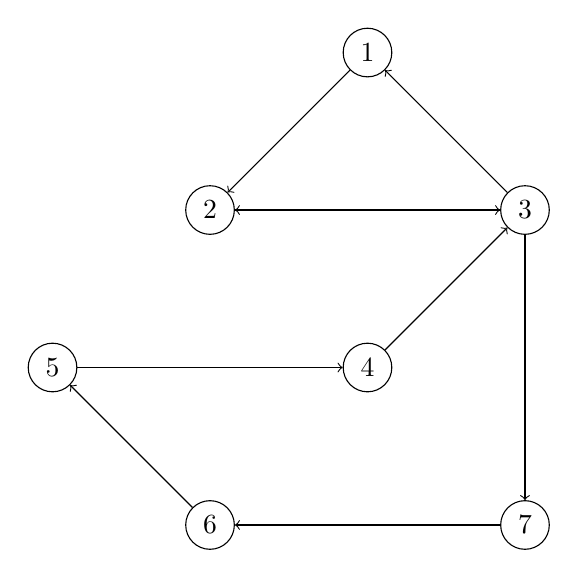
\begin{tikzpicture}
\node[shape=circle,draw=black] (1) at (0,0) {\(\paren{1}\)};
\node[shape=circle,draw=black] (2) at (-2,-2) {\(\paren{2}\)};
\node[shape=circle,draw=black] (3) at (2,-2) {\(\paren{3}\)};
\node[shape=circle,draw=black] (4) at (0,-4) {\(\paren{4}\)};
\node[shape=circle,draw=black] (5) at (-4,-4) {\(\paren{5}\)};
\node[shape=circle,draw=black] (6) at (-2,-6) {\(\paren{6}\)};
\node[shape=circle,draw=black] (7) at (2,-6) {\(\paren{7}\)};
\path[->] (1) edge (2);
\path[->] (2) edge (3);
\path[->] (3) edge (1);
\path[->] (3) edge (2);
\path[->] (3) edge (7);
\path[->] (7) edge (6);
\path[->] (6) edge (5);
\path[->] (5) edge (4);
\path[->] (4) edge (3);
\end{tikzpicture}
\end{center}
\end{dem}

\begin{exo}\thlabel{exo1.18}
On pose \(E=\ensclasse{0}{\intervii{0}{1}}{\R}\) muni de la norme infinie.

L'application \(f\mapsto\int_0^1f\paren{t}\odif{t}\) est-elle continue sur \(E\) ?
\end{exo}

\begin{corr}
Pour \(f\in E\), on a \(\norme{f}_\infty=\sup_{\intervii{0}{1}}\abs{f}\in\R\) car \(\abs{f}\) est continue sur le segment \(\intervii{0}{1}\).

On note \(I:f\mapsto\int_0^1f\paren{t}\odif{t}\). \(I\) est linéaire.

Pour \(f\in E\), on a \(\abs{I\paren{f}}\leq\int_0^1\abs{f}\).

Or \(\quantifs{\forall t\in\intervii{0}{1}}\abs{f\paren{t}}\leq\norme{f}_\infty\).

Donc \[\abs{I\paren{f}}\leq\int_0^1\abs{f}\leq\int_0^1\norme{f}_\infty\odif{t}=\norme{f}_\infty.\]

Donc d'après la \thref{prop1.22}, \(I\) est continue sur \(E\).
\end{corr}

\begin{exo}
\(E\) désigne le même espace et on pose \(\norme{f}_1=\int_0^1\abs{f\paren{t}}\odif{t}\).

Montrez que \(\norme{}_1\) est une norme sur \(E\).

L'application \(f\mapsto f\paren{1}\) est-elle continue sur \(E\) ?
\end{exo}

\begin{corr}[\(\norme{}_1\) est une norme sur \(E\)]~\\
\begin{itemize}
    \item Soit \(f\in E\). Si \(\norme{f}_1=0\) alors \(\int_0^1\abs{f}=0\). Or \(\abs{f}\) est continue et positive donc d'après le théorème de stricte positivité de l'intégrale, \(\abs{f}=0\) donc \(f=0\). \\
    \item Soient \(f\in E\) et \(\lambda\in\R\). On a \[\norme{\lambda f}_1=\int_0^1\abs{\lambda f}=\int_0^1\abs{\lambda}\abs{f}=\abs{\lambda}\int_0^1\abs{f}=\abs{\lambda}\norme{f}_1.\]
    \item Soit \(\paren{f,g}\in E^2\). On a \[\norme{f+g}_1=\int_0^1\abs{f+g}\leq\int_0^1\paren{\abs{f}+\abs{g}}=\int_0^1\abs{f}+\int_0^1\abs{g}=\norme{f}_1+\norme{g}_1.\]
    \item Donc \(\norme{}_1\) est une norme sur \(E\).
\end{itemize}
\end{corr}

\begin{corr}[Continuité de l'application ?]
On pose \(\fonction{V}{E}{\R}{f}{f\paren{1}}\)

Pour \(n\in\Ns\), on pose \(f_n:x\mapsto\begin{dcases}
0 &\text{si }x\in\intervii{0}{1-\dfrac{1}{n}} \\
n^2\paren{x-\paren{1-\dfrac{1}{n}}} &\text{sinon}
\end{dcases}\)

Pour \(n\in\Ns\), on a \(\int_0^1\abs{f}=\int_0^1f_n=\dfrac{1}{2}\) donc \(f_n\in\bouleo{0}{1}\).

Or \(\abs{V\paren{f_n}}=\abs{f_n\paren{1}}=n\tendqd{n\to\pinf}\pinf\).

On a ainsi trouvé une suite \(\paren{f_n}\) à termes dans \(\bouleo{0}{1}\) telle que \(V\paren{f_n}\tendqd{n\to\pinf}\pinf\).

Donc \(V\) n'est pas bornée sur \(\bouleo{0}{1}\).

Donc comme \(V\) est linéaire, \(V\) n'est pas continue sur \(\groupe{E}[\norme{}_1]\).

Remarque : on a \(\quantifs{\forall f\in E}\abs{V\paren{f}}=\abs{f\paren{1}}\leq\norme{f}_\infty\) donc \(V\) est continue sur \(\groupe{E}[\norme{}_\infty]\).
\end{corr}

\begin{defi}
On note \(\Lc{E}{F}\) l'ensemble des applications linéaires continues de \(E\) dans \(F\).
\end{defi}

\begin{prop}
\(\Lc{E}{F}\) est un sous-espace vectoriel de \(\L{E}{F}\), en général distinct de \(\L{E}{F}\).
\end{prop}

Cas particulier en dimension finie.

\begin{theo}
On suppose que \(E\) est de dimension finie.

Toute application linéaire de \(E\) dans \(F\) est lipschitzienne sur \(E\), donc continue.

Autrement dit, si \(E\) est de dimension finie, alors \(\Lc{E}{F}=\L{E}{F}\).
\end{theo}

\begin{dem}
On note \(p=\dim E\) et \(\fami{B}=\paren{e_1,\dots,e_p}\) une base de \(E\).

Pour \(x=\paren{x_1,\dots,x_p}_\fami{B}\), on a \(\norme{x}_\infty=\sup_{1\leq i\leq p}\abs{x_i}=\max_{1\leq i\leq p}\abs{x_i}\).

Soit \(f\in\L{E}{F}\) et \(N\) une norme sur \(F\).

Pour \(x=\paren{x_1,\dots,x_p}_\fami{B}\), on a \(x=\sum_{k=1}^px_ke_k\).

Donc, \(f\) étant linéaire, on a \(f\paren{x}=\sum_{k=1}^px_kf\paren{e_k}\).

Donc \[\begin{aligned}
N\paren{f\paren{x}}&=N\paren{\sum_{k=1}^px_kf\paren{e_k}} \\
&\leq\sum_{k=1}^pN\paren{x_kf\paren{e_k}} \\
&=\sum_{k=1}^p\abs{x_k}N\paren{f\paren{e_k}}.
\end{aligned}\]

De plus, on a \[\begin{aligned}
\quantifs{\forall i\in\interventierii{1}{p}}\abs{x_i}&\leq\norme{x}_\infty \\
\abs{x_i}N\paren{f\paren{e_i}}&\leq\norme{x}_\infty N\paren{f\paren{e_i}}.
\end{aligned}\]

Donc \(N\paren{f\paren{x}}\leq\norme{x}_\infty\underbrace{\sum_{k=1}^pN\paren{f\paren{e_k}}}_{K}\).

Ceci prouve d'après la \thref{prop1.22} que \(f\) est continue de \(\groupe{E}[\norme{}_\infty]\) dans \(\groupe{F}[N]\).

Soit maintenant \(\norme{}\) une norme quelconque sur \(E\).

Comme \(E\) est de dimension finie, toutes les normes sur \(E\) sont équivalentes, donc il existe \(a,b>0\) tels que \(a\norme{}\leq\norme{}_\infty\leq b\norme{}\).

Donc \(\quantifs{\tpt x\in E}N\paren{f\paren{x}}\leq bK\norme{x}\).

Donc \(f\) est continue de \(\groupe{E}[\norme{}]\) dans \(\groupe{F}[N]\).
\end{dem}

\begin{rem}
L'hypothèse de dimension finie de \(E\) est indispensable. Dans le cas contraire, c'est faux en général.
\end{rem}

Le résultat précédent s'étend aux applications multilinéaires.

\begin{theo}
Soient \(E_1,\dots,E_n\) des espaces vectoriels normés de dimensions finies et \(f:E_1\times\dots\times E_n\to F\) une application \(n\)-linéaire.

Il existe alors une constante \(K\geq0\) telle que \[\quantifs{\tpt\paren{x_1,\dots,x_n}\in E_1\times\dots\times E_n}\norme{f\paren{x_1,\dots,x_n}}\leq K\norme{x_1}_{E_1}\dots\norme{x_n}_{E_n}.\]
\end{theo}

\begin{dem}
Pour tout \(i\in\interventierii{1}{n}\), on note \(p_i=\dim E_i\) et \(\fami{B}_i=\paren{e_{i,1},\dots,e_{i,p_i}}\) une base de \(E_i\).

Soit \(\paren{x_1,\dots,x_n}\in E_1\times\dots\times E_n\). Pour tout \(i\in\interventierii{1}{n}\), on note \(x_i=\paren{x_{i,1},\dots,x_{i,p_i}}_{\fami{B}_i}\).

On a \[\begin{aligned}
f\paren{x_1,\dots,x_n}&=f\paren{\sum_{j_1=1}^{p_1}x_{1,j_1}e_{1,j_1},\dots,\sum_{j_n=1}^{p_n}x_{n,j_n}e_{n,j_n}} \\
&=\sum_{j_1=1}^{p_1}\dots\sum_{j_n=1}^{p_n}x_{1,j_1}\dots x_{n,j_n}f\paren{e_{1,j_1},\dots,e_{n,j_n}}.
\end{aligned}\]

Donc \[\begin{aligned}
N\paren{f\paren{x_1,\dots,x_n}}&\leq\sum_{\substack{1\leq j_1\leq p_1 \\ \vdots \\ 1\leq j_n\leq p_n}}\abs{x_{1,j_1}}\dots\abs{x_{n,j_n}}N\paren{f\paren{e_{1,j_1},\dots,e_{n,j_n}}} \\
&\leq\norme{x_1}_{1,\infty}\dots\norme{x_n}_{n,\infty}\underbrace{\sum_{\substack{1\leq j_1\leq p_1 \\ \vdots \\ 1\leq j_n\leq p_n}}N\paren{f\paren{e_{1,j_1},\dots,e_{n,j_n}}}}_{K}.
\end{aligned}\]

On conclut de la même façon que dans la démonstration précédente.
\end{dem}

\begin{cor}
Soient \(E_1,\dots,E_n\) des espaces vectoriels normés de dimensions finies.

Toute application \(f:E_1\times\dots\times E_n\to F\) qui est \(n\)-linéaire est continue sur \(E_1\times\dots\times E_n\).
\end{cor}

\begin{ex}
\begin{itemize}
    \item Le produit matriciel de \(\M{np}\times\M{pq}\) dans \(\M{nq}\) est bilinéaire, donc continu. \\
    \item Un produit scalaire dans un espace euclidien est bilinéaire, donc continu. \\
    \item Le déterminant dans \(\M{n}\) est \(n\)-linéaire par rapport aux colonnes, donc il est continu.
\end{itemize}
\end{ex}

\subsection{Norme subordonnée}

On définit sur l'espace vectoriel \(\Lc{E}{F}\) des applications linéaires continues de \(E\) dans \(F\) la notion de norme subordonnée (relative aux deux normes sur \(E\) et \(F\)) ou norme triple.

\begin{defi}
Soit \(f\in\Lc{E}{F}\).

On pose \(\normesub{f}=\sup_{x\in\bouleo{0}{1}}\norme{f\paren{x}}\), appelée la norme subordonnée de \(f\).
\end{defi}

\begin{rem}
Cette définition a un sens car \(f\) étant linéaire de \(E\) dans \(F\) et continue, elle est bornée sur \(\bouleo{0}{1}\) d'après la \thref{prop1.22}.
\end{rem}

\begin{rem}
On a \[\normesub{f}=\sup_{x\in\bouleo{0}{1}}\norme{f\paren{x}}=\sup_{x\in\sphere{0}{1}}\norme{f\paren{x}}=\sup_{x\in\boulef{0}{1}}\norme{f\paren{x}}.\]
\end{rem}

\begin{prop}
Soit \(f\in\Lc{E}{F}\).

Alors \(\normesub{f}\) est

\begin{itemize}
    \item égal à \(\sup_{x\not=0}\dfrac{\norme{f\paren{x}}}{\norme{x}}\), mais aussi à \(\sup_{x\in\sphere{0}{1}}\norme{f\paren{x}}\) ; \\
    \item le plus petit réel positif \(M\) tel que \(\quantifs{\tpt x\in E}\norme{f\paren{x}}\leq M\norme{x}\).
\end{itemize}
\end{prop}

\begin{dem}
On note \(N_1\paren{f}=\sup_{x\not=0}\dfrac{\norme{f\paren{x}}}{\norme{x}}\) et \(N_2\paren{f}=\sup_{x\in\sphere{0}{1}}\norme{f\paren{x}}\).
\end{dem}

\begin{dem}[\(N_1\paren{f}=N_2\paren{f}\)]~\\
\(\quantifs{\Tpt x\not=0}\dfrac{x}{\norme{x}}\in\sphere{0}{1}\).

Donc \(\norme{f\paren{\dfrac{x}{\norme{x}}}}\leq N_2\paren{f}\).

Donc \(\dfrac{1}{\norme{x}}\norme{f\paren{x}}\leq N_2\paren{f}\) \ie \(N_1\paren{f}\leq N_2\paren{f}\).

De plus, \(\quantifs{\tpt x\in\sphere{0}{1}}\norme{x}=1\) donc \(\dfrac{\norme{f\paren{x}}}{\norme{x}}=\norme{f\paren{x}}\leq N_1\paren{f}\).

Donc \(N_2\paren{f}\leq N_1\paren{f}\).

Finalement, on a \(N_1\paren{f}=N_2\paren{f}\).
\end{dem}

\begin{dem}[\(N_2\paren{f}=\normesub{f}\)]~\\
Pour tout \(x\in\bouleo{0}{1}\excluant\accol{0}\), on a \(\dfrac{x}{\norme{x}}\in\sphere{0}{1}\) donc \[\begin{aligned}
\norme{f\paren{\dfrac{x}{\norme{x}}}}&\leq N_2\paren{f} \\
\dfrac{1}{\norme{x}}\norme{f\paren{x}}&\leq N_2\paren{f}.
\end{aligned}\]

Or \(\norme{x}\leq1\) donc \(\norme{f\paren{x}}\leq\dfrac{1}{\norme{x}}\norme{f\paren{x}}\leq N_2\paren{f}\).

Ceci est encore vrai pour \(x=0\) donc \(\normesub{f}\leq N_2\paren{f}\).

De plus, soient \(x\in\sphere{0}{1}\) et \(\lambda\in\intervie{0}{1}\).

On a \(\norme{\lambda x}=\lambda<1\) donc \(\lambda x\in\bouleo{0}{1}\).

Donc \(\norme{f\paren{\lambda x}}=\lambda\norme{f\paren{x}}\leq\normesub{f}\).

Donc, par passage à la limite quand \(\lambda\to1\) : \[\norme{f\paren{x}}\leq\normesub{f}\] \ie \(N_2\paren{f}\leq\normesub{f}\).

Donc \(N_2\paren{f}=\normesub{f}\).
\end{dem}

\begin{dem}[Second point]
On a \[\begin{aligned}
\normesub{f}&=\sup_{x\not=0}\dfrac{\norme{f\paren{x}}}{\norme{x}} \\
&=\min\accol{K\in\R\tq\quantifs{\forall x\not=0}\dfrac{\norme{f\paren{x}}}{\norme{x}}\leq K} \\
&=\min\accol{K\in\R\tq\quantifs{\forall x\in E}\norme{f\paren{x}}\leq K\norme{x}}.
\end{aligned}\]
\end{dem}

\begin{ex}
Dans l'\thref{exo1.18}, on avait montré \(\quantifs{\forall f\in E}\abs{I\paren{f}}\leq\norme{f}_\infty\).

On a \(\abs{I\paren{1}}=1=1\times\norme{1}_\infty\).

Donc \(\normesub{I}=1\).
\end{ex}

\begin{meth}
Si \[\quantifs{\forall x\in E}\norme{f\paren{x}}\leq K\norme{x}\] et s'il existe \(x_0\in E\) tel que \[\norme{f\paren{x_0}}=K\norme{x_0}\] alors \(\normesub{f}=K\).
\end{meth}

\begin{prop}
Les normes subordonnées sont des normes sur les espaces \(\Lc{E}{F}\).

Elles sont dites sous-multiplicatives : pour toutes applications linéaires continues et composables \(f\) et \(g\), \[\normesub{f\rond g}\leq\normesub{f}\times\normesub{g}.\]
\end{prop}

\begin{dem}[\(\normesub{}\) est une norme sur \(\Lc{E}{F}\)]
\begin{itemize}
    \item Soit \(f\in\Lc{E}{F}\). \\\\ Si \(\normesub{f}=0\) alors \(\quantifs{\forall x\in E}\norme{f\paren{x}}\leq0\times\norme{x}\) donc \(f=0\). \\
    \item Soient \(f\in\Lc{E}{F}\) et \(\lambda\in\K\). \\\\ On a \[\normesub{\lambda f}=\sup_{x\not=0}\dfrac{\norme{\lambda f\paren{x}}}{\norme{x}}=\sup_{x\not=0}\abs{\lambda}\dfrac{\norme{f\paren{x}}}{\norme{x}}=\abs{\lambda}\sup_{x\not=0}\dfrac{\norme{f\paren{x}}}{\norme{x}}=\abs{\lambda}\normesub{f}.\]
    \item Soit \(\paren{f,g}\in\Lc{E}{F}^2\). \\\\ On a \[\begin{aligned}
        \quantifs{\forall x\in\bouleo{0}{1}}\norme{\paren{f+g}\paren{x}}&=\norme{f\paren{x}+g\paren{x}} \\
        &\leq\norme{f\paren{x}}+\norme{g\paren{x}} \\
        &\leq\normesub{f}+\normesub{g}
    \end{aligned}\] donc \(\normesub{f+g}\leq\normesub{f}+\normesub{g}\).
\end{itemize}
\end{dem}

\begin{dem}[Sous-multiplicativité]
On a \[\begin{aligned}
\quantifs{\forall x\in E}\norme{f\rond g\paren{x}}&=\norme{f\paren{g\paren{x}}} \\
&\leq\normesub{f}\norme{g\paren{x}} \\
&\leq\normesub{f}\normesub{g}\norme{x}.
\end{aligned}\]

Donc \(\normesub{f\rond g}\leq\normesub{f}\normesub{g}\).
\end{dem}

Comme en dimension finie, on peut représenter par choix de bases les applications linéaires par des matrices, on définit de manière semblable la notion de norme sous-multiplicative de matrices (relativement aux normes) ou norme triple.

\begin{defi}
Soit \(\paren{n,p}\in\paren{\Ns}^2\). On choisit deux normes sur \(\K^p\) et \(\K^n\) (espaces identifiés à ceux des matrices-colonnes).

Pour toute matrice \(A\in\M{np}\), on pose \(\normesub{A}=\sup_{\norme{X}=1}\norme{AX}\).
\end{defi}

\begin{prop}
Des normes étant choisies sur les espaces \(\K^p\) et \(\K^n\), les normes subordonnées sont des normes sur tous les espaces \(\M{np}\).

Elles sont dites sous-multiplicatives : pour toutes matrices multipliables \(A\) et \(B\), \[\normesub{AB}\leq\normesub{A}\times\normesub{B}.\]
\end{prop}

\begin{rem}
Dans le cas où un espace vectoriel normé \(E\) est aussi une \(\K\)-algèbre, on dit qu'il est une algèbre normée quand la norme vérifie en plus la propriété de sous-multiplicativité : \(\quantifs{\forall\paren{x,y}\in E^2}\norme{xy}\leq\norme{x}\cdot\norme{y}\).
\end{rem}

\begin{rem}
En dimension finie, toute \(\K\)-algèbre \(A\) possède des normes sous-multiplicatives.
\end{rem}

\begin{dem}
Soit \(A\) une \(\K\)-algèbre de dimension finie.

L'application \(\fonctionlambda{A^2}{A}{\paren{a,b}}{ab}\) est bilinéaire donc continue.

Il existe donc \(K>0\) tel que \[\quantifs{\forall\paren{a,b}\in A^2}\norme{ab}\leq K\norme{a}\norme{b}.\]

On pose \(N=K\norme{}\).

On a alors \[\quantifs{\forall\paren{a,b}\in A^2}N\paren{ab}\leq N\paren{a}N\paren{b}\] et \(N\) est une norme sur \(A\).
\end{dem}

\section{Topologie d'un espace vectoriel normé}

Dans cette section, \(E\) est un espace vectoriel normé.

\subsection{Intérieur d'une partie, voisinage d'un point}

\begin{defi}
Soient \(A\) une partie de \(E\) et \(a\in A\).

On dit que \(a\) est un point intérieur à \(A\) quand on peut trouver un rayon \(r>0\) tel que \(\bouleo{a}{r}\) soit incluse dans \(A\). On dit aussi dans ce cas que \(A\) est un voisinage de \(a\).

L'intérieur de \(A\) est l'ensemble de ses points intérieurs, noté \(\interieur{A}\).

On a : \[a\in\interieur{A}\ssi\quantifs{\exists r>0}\bouleo{a}{r}\subset A.\]
\end{defi}

\begin{exo}
Dans \(\R\), quels sont les intérieurs des parties suivantes : \(\intervii{0}{1}\), \(\intervie{0}{\pinf}\), \(\Q\) ?
\end{exo}

\begin{corr}
\begin{itemize}
    \item Si \(A=\intervii{0}{1}\), alors \(\interieur{A}=\intervee{0}{1}\). \\\\ En effet, pour \(x\in\intervee{0}{1}\), on peut poser \(r=\min\paren{\dfrac{x}{2},\dfrac{1-x}{2}}>0\) pour avoir \(\bouleo{x}{r}\subset\intervii{0}{1}\). \\
    \item Si \(A=\intervie{0}{\pinf}\), alors \(\interieur{A}=\intervee{0}{\pinf}\) (même idée). \\
    \item Si \(A=\Q\), alors \(\interieur{A}=\ensvide\). \\\\ En effet, \(\quantifs{\tpt x\in\Q;\tpt r>0}\text{il existe }y\in\R\excluant\Q\) tel que \(\abs{x-y}<r\) \ie \(\bouleo{x}{r}\not\subset\Q\).
\end{itemize}
\end{corr}

\begin{exo}
Quel est l'intérieur d'une boule de centre \(a\) et de rayon \(r>0\) ?
\end{exo}

\begin{corr}
Soient \(a\in E\) et \(r>0\).

Si \(A=\bouleo{a}{r}\), alors \(\interieur{A}=A\).

En effet, pour tout \(x\in\bouleo{a}{r}\), on pose \(p=\dfrac{r-\norme{x-a}}{2}>0\) et on a \[\bouleo{x}{p}\subset A.\]
\end{corr}

\begin{rem}
Cette notion dépend a prori de la norme utilisée. En dimension finie, ce n'est pas le cas : l'intérieur d'une partie d'un espace vectoriel normé de dimension finie ne dépend pas du choix de la norme (pourquoi ?).
\end{rem}

\begin{dem}
Si \(N_1,N_2\) sont deux normes équivalentes sur \(E\), \(A\) est une partie de \(E\) et \(a\in E\), alors \(a\) est intérieur à \(A\) pour \(N_1\) ssi \(a\) est intérieur à \(A\) pour \(N_2\).

Il existe \(\alpha,\beta>0\) tels que \(\alpha N_2\leq N_1\leq\beta N_2\).

Si \(a\) est intérieur à \(A\) pour \(N_1\), alors il existe \(r>0\) tel que \(\bouleo[1]{a}{r}\subset A\).

On pose \(p=\dfrac{r}{\beta}>0\) et on montre \(\bouleo[2]{a}{p}\subset A\).

Soit \(x\in\bouleo[2]{a}{p}\).

On a \(N_2\paren{a-x}<p=\dfrac{r}{\beta}\).

Donc \(N_1\paren{a-x}\leq\beta N_2\paren{a-x}<r\).

Donc \(x\in\bouleo[1]{a}{r}\subset A\).

Donc \(x\) est intérieur à \(A\) pour \(N_2\).

On montre la réciproque de même, en montrant \(\bouleo[1]{a}{\alpha r}\subset\bouleo[2]{a}{r}\).
\end{dem}

\begin{prop}
Soient \(u\in E^\N\) et \(l\in E\).

La suite \(u\) converge vers \(l\) ssi tout voisinage de \(l\) contient tous les termes de la suite à partir d'un certain rang.
\end{prop}

\subsection{Parties ouvertes}

\begin{defi}
On dit qu'une partie \(A\) de \(E\) est ouverte (ou est un ouvert) quand à tout point de \(a\in A\), on peut associer un rayon \(r>0\) tel que la boule de centre \(a\) et de rayon \(r\) soit incluse dans \(A\) : \[\quantifs{\forall a\in A;\exists r>0}\bouleo{a}{r}\subset A.\]

Autrement dit, \(A\) est ouverte quand tout point de \(A\) est intérieur à \(A\) : \(A=\interieur{A}\), ou, autrement dit, quand \(A\) est un voisinage de chacun de ses points.
\end{defi}

\begin{prop}
L'ensemble vide et \(E\) sont des parties ouvertes. Toute boule ouverte est une partie ouverte. Tout produit (fini) de parties ouvertes est ouvert.
\end{prop}

\begin{dem}
Soient \(E,F\) deux esapces vectoriels normés par \(\norme{}_E\) et \(\norme{}_F\).

On pose \(N\paren{x,y}=\max\paren{\norme{x}_E,\norme{y}_F}\) pour obtenir une norme \(N\) sur \(E\times F\).

Montrons que si \(A\) est un ouvert de \(E\) et \(B\) un ouvert de \(F\), alors \(A\times B\) est un ouvert de \(E\times F\).

Soit \(\paren{a,b}\in A\times B\).

\(a\in A\) et \(A\) est un ouvert donc il existe \(r>0\) tel que \(\bouleo[E]{a}{r}\subset A\).

\(b\in B\) et \(B\) est un ouvert donc il existe \(s>0\) tel que \(\bouleo[F]{b}{s}\subset B\).

On pose \(p=\min\paren{r,s}>0\).

Montrons que \(\bouleo[E\times F]{\paren{a,b}}{p}\subset A\times B\).

Soit \(\paren{x,y}\in\bouleo[E\times F]{\paren{a,b}}{p}\).

On a \(N\paren{\paren{x,y}-\paren{a,b}}<p\) \ie \(N\paren{x-a,y-b}<p\).

Donc \(\norme{x-a}_E<p\) et \(\norme{y-b}_F<p\).

Donc \(x\in\bouleo[E]{a}{p}\) et \(y\in\bouleo[F]{b}{p}\).

Or \(p\leq r\) donc \(\bouleo[E]{a}{p}\subset\bouleo[E]{a}{r}\subset A\) et \(p\leq s\) donc \(\bouleo[F]{b}{p}\subset\bouleo[F]{b}{s}\subset B\).

Donc \(\paren{x,y}\in A\times B\).

Donc \(\bouleo[E\times F]{\paren{a,b}}{p}\subset A\times B\).

On généralise à un produit de plusieurs ouverts par récurrence.
\end{dem}

La topologie de \(E\) est l'ensemble de tous les ouverts de \(E\).

\begin{rem}
La topologie dépend a priori de la norme utilisée. En dimension finie, ce n'est pas le cas : dans un espace vectoriel normé de dimension finie, le fait d'être un ouvert ne dépend pas du choix de la norme.
\end{rem}

\subsection{Parties fermées}

On rappelle la notion de point adhérent à une partie.

\begin{defi}
Soient \(A\) une partie de \(E\) et \(x\in E\).

On dit que \(x\) est un point adhérent à \(A\) quand il existe une suite \(u\in A^\N\) qui converge vers \(x\), ou, ce qui revient au même, quand toute boule centrée en \(x\) rencontre \(A\), ou encore quand \(d\paren{x,A}=0\).

L'adhérence de \(A\) est l'ensemble de ses points adhérents, noté \(\conj{A}\).
\end{defi}

On a montré

\begin{defi}
On dit qu'une partie \(A\) de \(E\) est fermée (ou est un fermé) quand tout point adhérent à \(A\) est dans \(A\), autrement dit quand la propriété suivante est vraie : \[\text{si une suite quelconque à termes dans }A\text{ converge vers un point }x\text{ de }E\text{, alors }x\in A.\]

Ou encore : \(A\) est fermée quand \(A=\conj{A}\).
\end{defi}

\begin{prop}
L'ensemble vide et \(E\) sont des parties fermées. Toute boule fermée est une partie fermée. Tout produit (fini) de parties fermées est fermé.
\end{prop}

On note le lien avec les parties ouvertes.

\begin{prop}
Soit \(A\) une partie de \(E\).

Alors \(A\) est une partie ouverte ssi son complémentaire est une partie fermée.
\end{prop}

\begin{dem}
\impdir

On suppose \(A\) ouverte. On veut montrer que \(E\excluant A\) est fermée.

Soit \(\paren{x_n}\in\paren{E\excluant A}^\N\) qui converge vers \(l\).

Par l'absurde, supposons \(l\in A\).

\(A\) est ouverte donc il existe \(\epsilon>0\) tel que \(\bouleo{l}{\epsilon}\subset A\).

Or \(x_n\tendqd{n\to\pinf}l\) donc il existe \(N\in\N\) tel que \[\quantifs{\forall n\geq N}x_n\in\bouleo{l}{\epsilon}.\]

Donc \(\quantifs{\tpt n\geq N}x_n\in A\) : contradiction.

Donc \(l\in E\excluant A\).

Donc \(E\excluant A\) est un fermé.

\imprec

Supposons que \(E\excluant A\) est fermée. On veut montrer que \(A\) est ouverte.

Soit \(a\in A\).

Par l'absurde, on suppose \(\quantifs{\forall r>0;\exists x\in\bouleo{a}{r}}x\not\in A\).

Alors pour tout \(n\in\N\), il existe \(x_n\in\bouleo{a}{\dfrac{1}{n+1}}\) tel que \(x_n\not\in A\).

On a construit une suite \(\paren{x_n}\in\paren{E\excluant A}^\N\) telle que \(\quantifs{\forall n\in\N}\norme{a-x_n}<\dfrac{1}{n+1}\).

Par théorème d'encadrement, on a \(x_n\tendqd{n\to\pinf}a\).

Or \(a\not\in E\excluant A\) : contradiction car \(E\excluant A\) est un fermé.

Donc il existe \(r>0\) tel que \(\bouleo{a}{r}\subset A\).

Donc \(A\) est un ouvert.
\end{dem}

Encore une fois, le fait d'être un fermé en dimension finie ne dépend pas de la norme.

\begin{prop}
\begin{itemize}
    \item Toute réunion de parties ouvertes est ouverte. Toute intersection finie de parties ouvertes est ouverte. \\
    \item Toute intersection de parties fermées est fermée. Toute réunion finie de parties fermées est fermée.
\end{itemize}
\end{prop}

\begin{dem}[Réunion d'ouverts]
Soit \(\paren{A_i}_{i\in I}\) une famille de parties ouvertes.

Montrons que \(\bigunion_{i\in I}A_i\) est ouverte.

Soit \(x\in\bigunion_{i\in I}A_i\).

Il existe \(i\in I\) tel que \(x\in A_i\).

Or \(A_i\) est ouverte donc il existe \(r>0\) tel que \(\bouleo{x}{r}\subset A_i\).

Donc \(\bouleo{x}{r}\subset\bigunion_{i\in I}A_i\).
\end{dem}

\begin{dem}[Intersection finie d'ouverts]
Soient \(A_1,\dots,A_n\) des parties ouvertes.

Montrons que \(\biginter_{i=1}^nA_i\) est ouverte.

Soit \(x\in\biginter_{i=1}^nA_i\).

Pour tout \(i\in\interventierii{1}{n}\), il existe \(r_i>0\) tel que \(\bouleo{x}{r_i}\subset A_i\).

On pose \(r=\min_{1\leq i\leq n}r_i>0\).

\(\quantifs{\Tpt i\in\interventierii{1}{n}}\bouleo{x}{r}\subset\bouleo{x}{r_i}\subset A_i\).

Donc \(\bouleo{x}{r}\subset\biginter_{i=1}^nA_i\).
\end{dem}

\begin{rem}
Si la famille d'ouverts n'est pas finie, on ne peut rien dire sur l'intersection.

Par exemple, pour \(n\in\N\), on pose les ouverts \(A_n=\intervee{\dfrac{-1}{n+1}}{\dfrac{1}{n+1}}\).

Alors \(\biginter_{n\in\N}A_n=\accol{0}\) n'est pas ouverte.
\end{rem}

\begin{exo}
Montrez que pour tout \(a\in E\), \(E\excluant\accol{a}\) est un ouvert. Déduisez-en que si \(A\) est une partie finie de \(E\), alors \(E\excluant A\) est un ouvert.
\end{exo}

\begin{corr}
Pour tout \(x\in E\excluant\accol{a}\), on pose \(r=\dfrac{\norme{x-a}}{2}\).

Alors \(\bouleo{x}{r}\subset E\excluant\accol{a}\).

Donc \(E\excluant\accol{a}\) est un ouvert.

Si \(A=\accol{a_1,\dots,a_n}\), alors \(E\excluant A\) est le complémentaire de \(\bigunion_{i=1}^n\accol{a_i}\), qui est un fermé par union finie de fermés, et est donc un ouvert.
\end{corr}

\begin{exo}
Quels sont les sous-espaces vectoriels de \(E\) qui sont ouverts ?
\end{exo}

\begin{corr}
Soit \(F\) un sous-espace vectoriel de \(E\) ouvert dans \(E\).

\(0\in F\) et \(F\) est un ouvert donc il existe \(r>0\) tel que \(\bouleo{0}{r}\subset F\).

Soit \(x\in E\excluant\accol{0}\).

On a \(\dfrac{r}{2}\dfrac{x}{\norme{x}}\in\bouleo{0}{r}\) donc \[x=\dfrac{2\norme{x}}{r}\paren{\dfrac{r}{2}\dfrac{x}{\norme{x}}}\in F.\]

Donc \(E=F\) : \(E\) est le seul sous-espace vectoriel de \(E\) ouvert dans \(E\).
\end{corr}

\begin{exo}
Montrez que \(F=\accol{\paren{x,y}\in\R^2\tq x\geq0\text{ et }xy=1}\) est un fermé de \(\R^2\).
\end{exo}

\begin{corr}
Soit \(\paren{\paren{x_n,y_n}}\in F^\N\) qui converge vers \(\paren{a,b}\).

Montrons que \(\paren{a,b}\in F\).

On a \(x_n\tendqd{n\to\pinf}a\), \(y_n\tendqd{n\to\pinf}b\) et \(\quantifs{\forall n\in\N}x_ny_n=1\).

Donc par passage à la limite quand \(n\to\pinf\), on a \(a\geq0\) et \(ab=1\).

Donc \(\paren{a,b}\in F\).

Donc \(F\) est un fermé.
\end{corr}

\begin{exo}
On note \(S\) l'ensemble des matrices de \(\M{n}[\R]\) telles que tous les coefficients soient positifs et sur chaque ligne la somme des coefficients vaut \(1\).

Montrez que \(S\) est un fermé.

NB : \(S\) est l'ensemble des matrices dites stochastiques.
\end{exo}

\begin{rem}
A priori, une partie de \(E\) n'est ni ouverte ni fermée : par exemple, dans \(\R\), l'ensemble \(\intervei{0}{1}\) n'est ni ouvert ni fermé.

Donc ne pas confondre \guillemets{complémentaire} et \guillemets{contraire} : on peut dire qu'une partie est un fermé quand son complémentaire est un ouvert, mais pas que le contraire d'être un ouvert c'est être un fermé.
\end{rem}

\begin{rem}
Il est souvent assez facile de montrer qu'une partie est un fermé grâce à la caractérisation séquentielle. Donc pour montrer qu'une partie est un ouvert, on montre souvent de cette façon que son complémentaire est un fermé.

Les fermés sont souvent définis par des égalités ou des inégalités larges. Par complémentaire, les ouverts sont souvent définis par des inégalités strictes ou des différences.
\end{rem}

\subsection{Ouverts ou fermés relatifs à une partie}

Les définitions précédentes parlent d'ouverts et de fermés de \(E\). On peut définir ces notions relativement à une partie.

\begin{defi}
Soient \(A\) une partie de \(E\) et \(U\) un sous-ensemble de \(A\).

On dit que \(U\) est un ouvert de \(A\) quand il existe un ouvert \(V\) de \(E\) tel que \(U=A\inter V\).

On dit que \(U\) est un fermé de \(A\) quand il existe un fermé \(V\) de \(E\) tel que \(U=A\inter V\).
\end{defi}

On remarque que les fermés de \(A\) sont les complémentaires dans \(A\) des ouverts de \(A\). On peut caractériser de même une partie \(U\) fermée de \(A\) par l'égalité entre \(U\) et l'ensemble de ses points adhérents dans \(A\).

\subsection{Image réciproque d'un ouvert ou d'un fermé par une fonction continue}

\begin{rappel}
Si \(f\) est une fonction de \(E\) dans \(F\) définie sur \(D_f\) et \(B\subset F\), l'image réciproque de \(B\) par \(f\) est \[f\inv\paren{B}=\accol{x\in D_f\tq f\paren{x}\in B}.\]
\end{rappel}

\begin{theo}
Soit \(f\) une fonction de \(E\) dans \(F\) définie sur \(D\).

Alors on a équivalence entre les propositions suivantes :

\begin{enumerate}
    \item \(f\) est continue sur \(D\) ; \\
    \item pour tout fermé \(B\) de \(F\), son image réciproque \(f\inv\paren{B}\) est un fermé de \(D\) ; \\
    \item pour tout ouvert \(B\) de \(F\), son image réciproque \(f\inv\paren{B}\) est un ouvert de \(D\).
\end{enumerate}

Ceci est valable en particulier quand \(f\) est une application continue de \(E\) dans \(F\), auquel cas on peut se passer des notions d'ouvert ou fermé relatif.
\end{theo}

\begin{dem}[\(\paren{1}\imp\paren{2}\)]
Soient \(B\) un fermé de \(F\) et \(\paren{u_n}\in f\inv\paren{B}^\N\) telle que \(u_n\tendqd{n\to\pinf}l\in D\).

\(f\) étant continue sur \(D\) et donc en \(l\), on a \(f\paren{u_n}\tendqd{n\to\pinf}f\paren{l}\).

De plus, on a \(\paren{f\paren{u_n}}\in B^\N\) or \(B\) est un fermé donc \(f\paren{l}\in B\).

Donc \(l\in f\inv\paren{B}\).

Donc \(f\inv\paren{B}\) est un fermé de \(D\).
\end{dem}

\begin{dem}[\(\paren{2}\imp\paren{3}\)]
Soit \(A\) un ouvert de \(F\).

Alors \(F\excluant A\) est un fermé de \(F\).

Donc \(f\inv\paren{F\excluant A}\) est un fermé de \(D\).

Or \(f\inv\paren{F\excluant A}=D\excluant f\inv\paren{A}\).

Donc \(f\inv\paren{A}\) est un ouvert de \(D\).
\end{dem}

\begin{dem}[\(\paren{3}\imp\paren{1}\)]
On suppose que \(\quantifs{\tpt A\text{ ouvert de }F}f\inv\paren{A}\) est un ouvert de \(D\).

Soit \(d\in D\). Montrons que \(f\) est continue en \(d\).

Soit \(\epsilon>0\).

La boule \(\bouleo{f\paren{d}}{\epsilon}\) est un ouvert de \(F\).

Donc \(f\inv\paren{\bouleo{f\paren{d}}{\epsilon}}\) est un ouvert de \(D\).

Or \(f\paren{d}\in\bouleo{f\paren{d}}{\epsilon}\) donc \(d\in f\inv\paren{\bouleo{f\paren{d}}{\epsilon}}\).

Donc il existe \(\alpha>0\) tel que \(D\inter\bouleo{d}{\alpha}\subset f\inv\paren{\bouleo{f\paren{d}}{\epsilon}}\).

Donc pour tout \(x\in D\) tel que \(x\in\bouleo{d}{\alpha}\), on a \(f\paren{x}\in\bouleo{f\paren{d}}{\epsilon}\) \ie \[\quantifs{\forall x\in D}\norme{x-d}<\alpha\imp\norme{f\paren{x}-f\paren{d}}<\epsilon.\]

Donc \(f\) est continue en \(d\).
\end{dem}

\begin{ex}[Cas particuliers fondamentaux]
Si \(f\) est continue sur \(E\) et à valeurs réelles, alors pour tout \(a\in\R\), les ensembles suivants sont des fermés de \(E\) : \[\accol{x\in E\tq f\paren{x}\geq a}\qquad\accol{x\in E\tq f\paren{x}\leq a}\qquad\accol{x\in E\tq f\paren{x}=a}.\]
\end{ex}

\begin{ex}
\begin{itemize}
    \item Les courbes de fonctions continues de \(\R\) dans \(\R\) sont des fermés de \(\R^2\). \\
    \item L'ensemble des matrices de trace nulle est un fermé de \(\M{n}\).
\end{itemize}
\end{ex}

\begin{dem}[Courbes des fonctions continues]
Si \(f:\R\to\R\) est continue, on pose \(\graphe{f}=\accol{\paren{x,y}\in\R^2\tq y=f\paren{x}}\).

On a alors \[\graphe{f}=\phi\inv\paren{\accol{0}}\] où \(\fonction{\phi}{\R^2}{\R}{\paren{x,y}}{y-f\paren{x}}\) est continue sur \(\R^2\) car \(f\) est continue sur \(\R\).

Or \(\accol{0}\) est un fermé de \(\R\) donc \(\graphe{f}\) est un fermé de \(\R^2\).
\end{dem}

\begin{dem}[Ensemble des matrices de trace nulle]
L'ensemble des matrices de trace nulle dans \(\M{n}\) est \[T=\accol{M\in\M{n}\tq\tr\paren{M}=0}.\]

Or \(\M{n}\) est de dimension finie et \(\tr\) est linéaire donc \(\tr\) est continue.

Donc \(T\) est l'image réciproque du fermé \(\accol{0}\) par l'application continue \(\tr\).

Donc \(T\) est un fermé de \(\M{n}\).
\end{dem}

Par passage au complémentaire, si \(f\) est continue sur \(E\) et à valeurs réelles, alors pour tout \(a\in\R\), les ensembles suivants sont des ouverts de \(E\) : \[\accol{x\in E\tq f\paren{x}<a}\qquad\accol{x\in E\tq f\paren{x}>a}\qquad\accol{x\in E\tq f\paren{x}\not=a}.\]

\begin{ex}
\begin{itemize}
    \item L'ensemble des couples \(\paren{x,y}\in\R^2\) tels que \(x>0\) et \(y>x\) est un ouvert de \(\R^2\). \\
    \item \(\GL{n}\) est un ouvert de \(\M{n}\) : si une matrice \(A\) est inversible, alors toutes les matrices proches de \(A\) le sont aussi.
\end{itemize}
\end{ex}

\begin{dem}[Ensemble des couples susmentionnés]
On pose \[\begin{aligned}
A&=\accol{\paren{x,y}\in\R^2\tq x>0\text{ et }y>x} \\
&=\accol{\paren{x,y}\in\R^2\tq x\in\intervee{0}{\pinf}}\inter\accol{\paren{x,y}\in\R^2\tq y-x\in\intervee{0}{\pinf}}.
\end{aligned}\]

Or \(\paren{x,y}\mapsto x\) et \(\paren{x,y}\mapsto y-x\) sont continues.

Donc \(A\) est un ouvert de \(\R^2\).
\end{dem}

\begin{dem}[\(\GL{n}\)]
On a \(\GL{n}={\det}\inv\paren{\K\excluant\accol{0}}\).

Or \(\det\) est continue et \(\K\excluant\accol{0}\) est un ouvert de \(\K\) donc \(\GL{n}\) est un ouvert de \(\M{n}\).
\end{dem}

\subsection{Frontière d'une partie}

\begin{defi}
Soit \(A\) une partie de \(E\). On appelle frontière de \(A\) l'ensemble \(\conj{A}\excluant\interieur{A}\).
\end{defi}

\begin{ex}
\begin{itemize}
    \item Si \(B\) est une boule, alors son intérieur est la boule ouverte de même centre et de même rayon, son adhérence est la boule fermée et sa frontière est la sphère. \\
    \item L'ensemble des rationnels est d'intérieur vide, d'adhérence égale à \(\R\) et donc de frontière \(\R\).
\end{itemize}
\end{ex}

\section{Compacité}

Dans cette section, \(E\) est un espace vectoriel normé.

\subsection{Valeurs d'adhérence d'une suite}

\begin{defi}
Soient \(u=\paren{u_n}\in E^\N\) et \(a\in E\).

On dit que \(a\) est une valeur d'adhérence de la suite \(u\) quand il existe une extractrice \(\phi\) telle que la suite extraite \(\paren{u_{\phi\paren{n}}}\) converge vers \(a\).
\end{defi}

Une suite peut avoir une ou plusieurs valeurs d'adhérence ou ne pas avoir de valeur d'adhérence :

\begin{itemize}
    \item la suite \(\paren{n}_{n\in\N}\) n'a pas de valeur d'adhérence ; \\
    \item toute suite convergente possède une seule valeur d'adhérence : sa limite ; \\
    \item la suite \(u\) définie par \(u_{2n}=\dfrac{1}{n+1}\) et \(u_{2n+1}=1-\dfrac{1}{n+1}\) possède deux valeurs d'adhérence : \(0\) et \(1\) ; \\
    \item il est possible de numéroter les rationnels, autrement dit de créer une suite \(u\) qui prend exactement toutes les valeurs rationnelles dans \(\R\) : cette suite a pour valeurs d'adhérence tous les réels.
\end{itemize}

On peut donner une caractérisation équivalente sans passer par la notion de suite extraite.

\begin{prop}\thlabel{prop1.32}
Soient \(u=\paren{u_n}\in E^\N\) et \(a\in E\).

Alors \(a\) est une valeur d'adhérence de \(u\) ssi \(\quantifs{\tpt\epsilon>0}\accol{n\in\N\tq u_n\in\bouleo{a}{\epsilon}}\text{ est infini}\).
\end{prop}

\begin{dem}
\imprec

Supposons que \(\quantifs{\tpt\epsilon>0}\accol{n\in\N\tq u_n\in\bouleo{a}{\epsilon}}\) est infini.

On spécialise \(\epsilon\gets\dfrac{1}{k+1}\) pour \(k\in\N\).

L'ensemble \(\accol{n\in\N\tq u_n\in\bouleo{a}{1}}\) est infini donc non-vide. On choisit \(\phi\paren{0}\) un élément de cet ensemble.

L'ensemble \(\accol{n\in\N\tq u_n\in\bouleo{a}{\dfrac{1}{2}}}\) est infini donc il contient des entiers strictement supérieurs à \(\phi\paren{0}\) ; on en choisit un, qu'on note \(\phi\paren{1}\).

Si on suppose avoir construit \(\phi\paren{0}<\phi\paren{1}<\dots<\phi\paren{k}\) tels que \(u_{\phi\paren{0}}\in\bouleo{a}{1}\), \(u_{\phi\paren{1}}\in\bouleo{a}{\dfrac{1}{2}}\), ..., \(u_{\phi\paren{k}}\in\bouleo{a}{\dfrac{1}{k+1}}\), comme l'ensemble \[\accol{n\in\N\tq u_n\in\bouleo{a}{\dfrac{1}{k+2}}}\] est infini, on peut choisir \(\phi\paren{k+1}\) dans cet ensemble tel que \(\phi\paren{k+1}>\phi\paren{k}\).

Par récurrence, on construit une suite \(\paren{\phi\paren{k}}_{k\in\N}\) strictement croissante d'entiers naturels tels que \[\quantifs{\forall k\in\N}u_{\phi\paren{k}}\in\bouleo{a}{\dfrac{1}{k+1}}\] \ie \(\norme{u_{\phi\paren{k}}-a}<\dfrac{1}{k+1}\).

Par théorème d'encadrement, on a \(u_{\phi\paren{k}}\tendqd{k\to\pinf}a\) : \(a\) est une valeur d'adhérence de la suite \(\paren{u_n}\).

\impdir

Supposons que \(a\) est une valeur d'adhérence de la suite \(\paren{u_n}\).

Il existe alors une extractrice \(\phi\) telle que \(u_{\phi\paren{k}}\tendqd{k\to\pinf}a\).

Donc pour tout \(\epsilon>0\), il existe \(N\in\N\) tel que \[\quantifs{\forall n\geq N}\norme{u_{\phi\paren{n}}-a}<\epsilon.\]

Donc \(\accol{n\in\N\tq u_n\in\bouleo{a}{\epsilon}}\) contient \(\phi\paren{N},\phi\paren{N+1},\dots\) \ie c'est un ensemble infini.
\end{dem}

Ceci peut encore être réécrit de la façon suivante.

\begin{prop}
Soient \(u=\paren{u_n}\in E^\N\) et \(a\in E\).

Alors \(a\) est une valeur d'adhérence de \(u\) ssi \(\quantifs{\forall\epsilon>0;\forall N\in\N;\exists n\geq N}\norme{u_n-a}<\epsilon\).
\end{prop}

\begin{dem}
Soit \(I\) une partie de \(\N\).

On a \[\begin{aligned}
I\text{ est infini}&\ssi I\text{ n'est pas majorée} \\
&\ssi\non\paren{\quantifs{\exists N\in\N;\forall n\in I}n\leq N} \\
&\ssi\quantifs{\forall N\in\N;\exists n\in I}n>N.
\end{aligned}\]

Pour tout \(\epsilon>0\), on pose \(I_\epsilon=\accol{n\in\N\tq u_n\in\bouleo{a}{\epsilon}}\).

On a alors, d'après la \thref{prop1.32} : \[\begin{aligned}
a\text{ est une valeur d'adhérence de }u&\ssi\quantifs{\forall\epsilon>0}I_\epsilon\text{ est infini} \\
&\ssi\quantifs{\forall\epsilon>0;\forall N\in\N;\exists n\in I_\epsilon}n>N \\
&\ssi\quantifs{\forall\epsilon>0;\forall N\in\N;\exists n>N}\norme{u_n-a}<\epsilon.
\end{aligned}\]
\end{dem}

\begin{exo}
Soit \(u=\paren{u_n}\in E^\N\). Montrez que l'ensemble \(V\) des valeurs d'adhérence de la suite \(u\) est un fermé de \(E\) en utilisant les ensembles \(U_p=\accol{u_n\tq n\geq p}\).
\end{exo}

\begin{corr}
Soit \(a\in E\).

On a \[\begin{aligned}
a\in V&\ssi\quantifs{\forall\epsilon>0;\forall N\in\N;\exists x\in U_N}\norme{x-a}<\epsilon \\
&\ssi\quantifs{\forall\epsilon>0;\forall N\in\N}U_N\inter\bouleo{a}{\epsilon}\not=\ensvide \\
&\ssi\quantifs{\forall N\in\N;\forall\epsilon>0}U_N\inter\bouleo{a}{\epsilon}\not=\ensvide \\
&\ssi\quantifs{\forall N\in\N}a\in\conj{U_N} \\
&\ssi a\in\biginter_{N\in\N}\conj{U_N}.
\end{aligned}\]

Donc \(V=\biginter_{N\in\N}\conj{U_N}\).

\(V\) est donc un fermé par intersection de fermés.
\end{corr}

\subsection{Théorème de Bolzano-Weierstrass}

\begin{theo}
Si \(E\) est de dimension finie, alors toute suite bornée de \(E\) possède une valeur d'adhérence.
\end{theo}

\begin{dem}
On note \(\P{k}\) le prédicat \guillemets{si \(E\) est de dimension \(k\), alors toute suite bornée de \(E\) possède une valeur d'adhérence}.

\begin{itemize}
    \item Pour \(k=1\) : \\\\ On pose \(E=\Vect{e_1}\). \\\\ Si \(\paren{u_n}\) est une suite bornée de \(E\), en notant \(\paren{u_n}=\paren{\lambda_ne_1}\) où \(\paren{\lambda_n}\) est une suite bornée de \(\K\), d'après le théorème de Bolzano-Weierstrass dans \(\R\) ou \(\C\), \(\paren{\lambda_n}\) possède une valeur d'adhérence et donc \(\paren{u_n}\) aussi. \\\\ D'où \(\P{1}\). \\
    \item Soit \(k\in\Ns\) tel que \(\P{k}\) soit vraie. \\\\ Soit \(E\) de dimension \(k+1\). \\\\ On choisit une base \(\fami{B}=\paren{e_1,\dots,e_{k+1}}\) de \(E\). \\\\ Soit \(\paren{u_n}\in E^\N\) une suite bornée. \\\\ Alors les suites-coordonnées associées sont bornées. \\\\ Pour tout \(n\in\N\), on note \(u_n=\paren{u_{1,n},\dots,u_{k+1,n}}_\fami{B}\). \\\\ \(\paren{u_{k+1,n}}_{n\in\N}\) est une suite bornée de \(\K\) donc (même théorème) il existe une extractrice \(\phi\) telle que \(\paren{u_{k+1,\phi\paren{n}}}_{n\in\N}\) converge. \\\\ Pour tout \(n\in\N\), on pose \(v_n=\paren{u_{1,n},\dots,u_{k,n},0}_\fami{B}\). \\\\ \(\paren{v_{\phi\paren{n}}}_{n\in\N}\) est une suite de vecteurs de \(\Vect{e_1,\dots,e_k}\) et bornée donc par hypothèse de récurrence, il existe une extractrice \(\psi\) telle que \(\paren{v_{\phi\rond\psi\paren{n}}}_{n\in\N}\) converge. \\\\ De plus, \(\paren{u_{k+1,\phi\rond\psi\paren{n}}}_{n\in\N}\) converge car c'est une suite extraite d'une suite convergente. \\\\ Donc \(\paren{u_{\phi\rond\psi\paren{n}}}_{n\in\N}\) converge. \\\\ Donc \(\P{k+1}\) est vrai. \\
    \item Donc \(\quantifs{\tpt k\in\Ns}\P{k}\) est vrai.
\end{itemize}
\end{dem}

\begin{rem}
Ce théorème est faux en dimension infinie donc il faut bien mettre en valeur la dimension finie.
\end{rem}

On peut ajouter une précision au théorème précédent.

\begin{prop}
Si \(E\) est de dimension finie, alors toute suite bornée de \(E\) qui ne possède qu'une seule valeur d'adhérence est convergente vers cette valeur d'adhérence.
\end{prop}

\begin{dem}
Supposons \(E\) de dimension finie.

Soit \(\paren{u_n}\in E^\N\) une suite bornée qui admet une unique valeur d'adhérence \(l\).

Par l'absurde, on suppose que \(\paren{u_n}\) ne converge pas vers \(l\).

On a \[\quantifs{\exists\epsilon>0}\underbrace{\quantifs{\forall N\in\N;\exists n\geq N}\norme{u_n-l}\geq\epsilon}_{\accol{n\in\N\tq u_n\not\in\bouleo{l}{\epsilon}}\text{ infini}}.\]

En ordonnant les éléments de cet ensemble et en les notant \(\phi\paren{0}<\phi\paren{1}<\dots\), on construit une extractrice \(\phi\) telle que \[\quantifs{\forall n\in\N}u_{\phi\paren{n}}\not\in\bouleo{l}{\epsilon}.\]

Or \(\paren{u_{\phi\paren{n}}}\) est bornée et \(E\) est de dimension finie donc d'après le théorème de Bolzano-Weierstrass, il existe une extractrice \(\psi\) et \(l\prim\in E\) tels que \[u_{\phi\rond\psi\paren{n}}\tendqd{n\to\pinf}l\prim.\]

Or pour tout \(n\in\N\), \(u_{\phi\paren{n}}\) appartient au fermé \(E\excluant\bouleo{l}{\epsilon}\) donc \(l\prim\in E\excluant\bouleo{l}{\epsilon}\).

Donc \(l\prim\not=l\).

Donc \(l\prim=\lim_{n\to\pinf}u_{\phi\rond\psi\paren{n}}\) est une autre valeur d'adhérence de \(\paren{u_n}\) : contradiction.

Donc \(u_n\tendqd{n\to\pinf}l\).
\end{dem}

\subsection{Parties compactes}

\begin{defi}
Soit \(A\) une partie de \(E\).

On dit que \(A\) est une partie compacte de \(E\) (ou un compact de \(E\)) quand toute suite à termes dans \(A\) possède une valeur d'adhérence dans \(A\) (propriété dite de Bolzano-Weierstrass).
\end{defi}

\begin{ex}
\begin{itemize}
    \item Tout segment \(\intervii{a}{b}\) de \(\R\) est un compact et ce sont les seuls intervalles compacts. \(\intervii{0}{1}\union\intervii{2}{3}\) est compact. \\
    \item Dans \(\K^n\), tout pavé \(\prod_{i=1}^n\intervii{a_i}{b_i}\) est un compact. Plus généralement, un produit (fini) de compacts est compact.
\end{itemize}
\end{ex}

Les parties compactes sont donc celles dont on peut extraire des sous-suites convergentes. Un résultat précédent se généralise alors.

\begin{prop}
Si \(A\) est une partie compacte, alors toute suite de \(A\) qui ne possède qu'une seule valeur d'adhérence est convergente vers cette valeur d'adhérence.
\end{prop}

Un compact étant connu, il est facile d'en construire d'autres.

\begin{prop}
Si \(A\) est une partie compacte de \(E\), alors toute partie \(B\) fermée dans \(A\) est aussi compacte.
\end{prop}

\begin{dem}
Soient \(A\) une partie compacte de \(E\), \(B\) un fermé de \(A\) et \(\paren{u_n}\in B^\N\).

Comme \(B\subset A\), on a \(\paren{u_n}\in A^\N\).

\(A\) est compacte donc il existe une extractrice \(\phi\) et \(l\in A\) tels que \(u_{\phi\paren{n}}\tendqd{n\to\pinf}l\).

La suite \(\paren{u_{\phi\paren{n}}}\) est à termes dans \(B\) et converge vers \(l\) donc comme \(B\) est un fermé, on a \(l\in B\).

Ainsi, toute suite de \(B^\N\) possède une valeur d'adhérence dans \(B\) \ie \(B\) est un compact.
\end{dem}

Reconnaître si une partie est compacte n'est pas toujours facile. On dispose d'une condition nécessaire, qui est suffisante en dimension finie.

\begin{prop}
Soit \(A\) une partie de \(E\).

Si \(A\) est compacte, alors \(A\) est une partie fermée et bornée.
\end{prop}

\begin{dem}
\begin{itemize}
    \item Si \(A\) n'est pas bornée, alors pour tout \(n\in\N\), il existe \(a_n\in A\) tel que \(\norme{a_n}\geq n\). \\\\ Si \(\paren{a_n}\) possède une valeur d'adhérence dans \(A\), alors il existe une extractrice \(\phi\) et \(l\in A\) tels que \(a_{\phi\paren{n}}\tendqd{n\to\pinf}l\). \\\\ Alors \(\norme{a_{\phi\paren{n}}}\tendqd{n\to\pinf}\norme{l}\) : contradiction. \\\\ Donc \(A\) n'est pas compacte. \\
    \item Supposons que \(A\) est compacte. \\\\ Soit \(\paren{u_n}\in A^\N\) telle que \(u_n\tendqd{n\to\pinf}l\in E\). \\\\ \(A\) étant compacte, il existe \(\phi\) une extractrice et \(l\prim\in A\) tels que \(u_{\phi\paren{n}}\tendqd{n\to\pinf}l\prim\). \\\\ La suite \(\paren{u_{\phi\paren{n}}}\) est extraite de la suite convergente \(\paren{u_n}\) donc \(u_{\phi\paren{n}}\tendqd{n\to\pinf}l\). \\\\ Donc par unicité de la limite, on a \(l\prim=l\in A\). \\\\ Donc \(A\) est fermée.
\end{itemize}
\end{dem}

La réciproque est hélas fausse en général. Néanmoins, en dimension finie, elle est vraie.

\begin{prop}
Si \(E\) est de dimension finie, alors une partie de \(E\) est compacte ssi elle est fermée et bornée.
\end{prop}

\begin{rem}
En fait, il n'y a qu'en dimension finie que ce résultat est vrai. Un théorème de Riesz affirme que la boule-unité fermée d'un espace vectoriel normé est compacte ssi l'espace est de dimension finie, ce qui revient à dire que l'équivalence précédente n'est valable que dans un espace de dimension finie.

En dimension infinie, il se passe des choses vraiment étranges : les compacts sont des parties très petites et plates, par exemple, un compact est forcément d'intérieur vide. Heureusement, il est plus courant de travailler à notre niveau en dimension finie.
\end{rem}

\begin{ex}
\begin{itemize}
    \item L'ensemble des matrices stochastiques de \(\M{n}[\R]\) est un compact. \\
    \item La boule-unité fermée de \(E=\ensclasse{0}{\intervii{0}{1}}{\R}\) pour la norme infinie n'est pas compacte, car la suite des fonctions \(\paren{x\mapsto x^n}\) a pour seule valeur d'adhérence possible la fonction \(x\mapsto0\) si \(x\not=1\) et \(1\mapsto1\), qui n'est même pas dans l'espace \(E\).
\end{itemize}
\end{ex}

\begin{dem}[Matrices stochastiques]
On note \[S_n=\accol{M=\paren{m_{i,j}}\in\M{n}[\R]\tq\quantifs{\forall\paren{i,j}\in\interventierii{1}{n}^2}m_{i,j}\geq0\text{ et }\quantifs{\forall i\in\interventierii{1}{n}}\sum_{j=1}^nm_{i,j}=1}.\]

Soit \(M=\paren{m_{i,j}}\in S_n\).

\(\quantifs{\Tpt i\in\interventierii{1}{n}}\sum_{j=1}^nm_{i,j}\) est une somme de réels positifs qui vaut \(1\) donc \(\quantifs{\tpt j\in\interventierii{1}{n}}0\leq m_{i,j}\leq1\).

Donc \(\norme{M}_\infty\leq1\).

Donc \(S_n\) est bornée.

Soit \(\paren{M_k}=\paren{\paren{m_{i,j}^k}_{i,j}}_k\) une suite de matrices de \(S_n\) qui converge vers \(A=\paren{a_{i,j}}\in\M{n}[\R]\) : \[\quantifs{\forall\paren{i,j}\in\interventierii{1}{n}^2}m_{i,j}^k\tendqd{k\to\pinf}a_{i,j}.\]

Par passage à la limite quand \(k\to\pinf\) dans les deux conditions qui définissent \(S_n\), on obtient \[\quantifs{\forall\paren{i,j}\in\interventierii{1}{n}^2}a_{i,j}\geq0\qquad\text{et}\qquad\quantifs{\forall i\in\interventierii{1}{n}}\sum_{j=1}^na_{i,j}=1.\]

Donc \(A\in S_n\).

Donc \(S_n\) est fermée.

On aurait aussi pu considérer les fonctions continues sur \(\M{n}[\R]\) \[c_{i,j}:\paren{m_{i,j}}\mapsto m_{i,j}\qquad\text{et}\qquad s_i:\paren{m_{i,j}}\mapsto\sum_{j=1}^nm_{i,j}\] et remarquer que \[S_n=\biginter_{1\leq i,j\leq n}c_{i,j}\inv\paren{\intervie{0}{\pinf}}\inter\biginter_{i=1}^ns_i\inv\paren{\accol{1}}\] ce qui montre que \(S_n\) est un fermé par intersection de fermés.

Alors, comme \(\M{n}[\R]\) est de dimension finie, on en déduit que \(S_n\) est un compact de \(\M{n}[\R]\).
\end{dem}

\begin{dem}[Deuxième point]
On pose \(f_n:x\mapsto x^n\).

\(\quantifs{\Tpt n\in\N}\norme{f}_\infty=1\).

Si \(\paren{f_n}\) a une valeur d'adhérence \(g\in\boulef{0}{1}\), alors il existe une extractrice \(\phi\) telle que \(f_{\phi\paren{n}}\tendqd{n\to\pinf}g\) \ie \(\norme{f_{\phi\paren{n}}-g}_\infty\tendqd{n\to\pinf}0\).

Or \(\quantifs{\tpt x\in\intervii{0}{1}}\abs{f_{\phi\paren{n}}\paren{x}-g\paren{x}}\leq\norme{f_{\phi\paren{n}}-g}_\infty\).

Donc par encadrement, on a \(f_{\phi\paren{n}}\paren{x}\tendqd{n\to\pinf}g\paren{x}\).

Si \(x\in\intervie{0}{1}\), alors \(f_{\phi\paren{n}}\paren{x}=x^{\phi\paren{n}}\tendqd{n\to\pinf}0\).

Si \(x=1\), alors \(f_{\phi\paren{n}}\paren{x}=1\tendqd{n\to\pinf}1\).

Donc \(g:x\mapsto\begin{dcases}
0 &\text{si }x\in\intervie{0}{1} \\
1 &\text{sinon}
\end{dcases}\)

Or \(g\not\in E\) : contradiction de la compacité.
\end{dem}

Une application importante de la notion de compacité est le théorème suivant.

\begin{theo}
Tout sous-espace vectoriel de dimension finie de \(E\) est fermé.
\end{theo}

\begin{dem}
Soit \(F\) un sous-espace vectoriel de \(E\) de dimension finie.

Soit \(\paren{u_n}\in F^\N\) une suite convergente vers \(l\in E\).

Alors \(\paren{u_n}\) est bornée : il existe \(R>0\) tel que \(\quantifs{\forall n\in\N}u_n\in\boulef{0}{R}\).

Donc \(\quantifs{\forall n\in\N}u_n\in\boulef{0}{R}\inter F=\accol{x\in F\tq\norme{x}\leq R}=\boulef[F]{0}{R}\).

Donc \(\boulef[F]{0}{R}\) est un fermé borné de \(F\) et donc un compact de \(F\).

Il existe donc une extractrice \(\phi\) et \(a\in\boulef[F]{0}{R}\) tels que \(u_{\phi\paren{n}}\tendqd{n\to\pinf}a\).

Donc \(l=a\in F\).

Donc \(F\) est fermé.
\end{dem}

En dimension infinie, là encore il peut se passer des choses étranges : un sous-espace de \(E\) de dimension infinie peut être dense (et donc non-fermé s'il est différent de \(E\)).

\subsection{Théorème des bornes atteintes}

Le principal intérêt des compacts est de pouvoir généraliser un théorème de première année.

\begin{theo}
Soient \(E,F\) deux espaces vectoriels normés, \(A\) une partie de \(E\) et \(f:A\to F\).

Si \(f\) est continue sur \(A\) et \(A\) est compacte, alors \(f\paren{A}\) est compacte.
\end{theo}

\begin{dem}
On suppose que \(f\) est continue et que \(A\) est compacte.

Soit \(\paren{u_n}\in f\paren{A}^\N\).

\(\quantifs{\Tpt n\in\N}u_n\in f\paren{A}\) donc il existe \(v_n\in A\) tel que \(u_n=f\paren{v_n}\).

\(\paren{v_n}\in A^\N\) et \(A\) est compacte donc il existe une extractrice \(\phi\) et \(a\in A\) tels que \(v_{\phi\paren{n}}\tendqd{n\to\pinf}a\).

\(f\) est continue en \(a\) donc \(u_{\phi\paren{n}}=f\paren{v_{\phi\paren{n}}}\tendqd{n\to\pinf}f\paren{a}\in f\paren{A}\).

Donc \(f\paren{A}\) est compacte.
\end{dem}

On résume en disant que l'image continue d'un compact est un compact.

En particulier, toute fonction continue sur un compact est donc bornée. Dans le cas des fonctions numériques (\ie à valeurs dans \(\R\)), on peut même être plus précis.

\begin{theo}
Toute fonction continue sur un compact et à valeurs réelles est bornée et atteint ses bornes.

Autrement dit, si \(f:A\to\R\) est continue sur \(A\) et \(A\) est une partie compacte de \(E\), alors il existe \(\paren{a,b}\in A^2\) tel que \(\quantifs{\tpt x\in A}f\paren{a}\leq f\paren{x}\leq f\paren{b}\), ce qui revient à dire que \(f\) possède un minimum et un maximum sur \(A\).
\end{theo}

\begin{dem}
\(f\paren{A}\) est un fermé borné de \(\R\) donc possède un minimum et un maximum.
\end{dem}

\begin{rem}
Pour toute partie \(X\) bornée de \(\R\) non-vide, \(\sup X\) et \(\inf X\) sont dans l'adhérence de \(X\).
\end{rem}

\begin{rem}
Ce théorème est à rapprocher du théorème vu en première année : toute fonction de \(\R\) dans \(\R\) continue sur un segment est bornée et atteint ses bornes.

Néanmoins, le théorème de l'an dernier donnait un résultat un peu plus précis que celui de cette année car il donnait aussi l'image du segment, en précisant qu'il s'agissait aussi d'un segment, car il faisait aussi intervenir le théorème des valeurs intermédiaires.

Ici, dans la version proposée cette année, on ne peut rien dire de plus.
\end{rem}

\begin{exo}
Un exercice classique, à savoir refaire ! C'est la base de nombreux exercices.

Soient \(E\) de dimension finie et \(f:E\to\R\) continue et telle que \(f\paren{x}\) tende vers \(\pinf\) quand \(\norme{x}\) tend vers \(\pinf\). Montrez que \(f\) possède un minimum.

Exemple : dans le plan euclidien géométrique, on choisit trois points \(A,B,C\) ; montrez alors qu'il existe un point \(M\) du plan tel que la somme \(AM+BM+CM\) soit minimale.
\end{exo}

\begin{corr}[Cas général]
On a \(f\paren{0}\in\R\) donc il existe \(A>0\) tel que \(\quantifs{\forall x\in E}\norme{x}>A\imp f\paren{x}\geq f\paren{0}\).

Sur \(\boulef{0}{A}\), fermé borné d'un espace de dimension finie donc un compact, \(f\) est continue et y admet donc un minimum en \(x_0\) d'après le théorème des bornes atteintes.

Pour tout \(x\in E\),

\begin{itemize}
    \item si \(x\not\in\boulef{0}{A}\), alors \(f\paren{x}\geq f\paren{0}\geq f\paren{x_0}\) car \(0\in\boulef{0}{A}\) \\
    \item si \(x\in\boulef{0}{A}\), alors \(f\paren{x}\geq f\paren{x_0}\).
\end{itemize}

Donc \(f\paren{x_0}=\min_Ef\).
\end{corr}

\begin{corr}[Exemple]
On note \(\fami{P}\) le plan considéré.

On pose \(\fonction{f}{\fami{P}}{\R}{M\dcoords{x}{y}}{AM+BM+CM}\) qui est une fonction continue.

Par inégalité triangulaire, on a \(f\paren{M}\geq3OM+\mathrm{cte}\) donc \[f\paren{M}\tendqd{\norme{\overrightarrow{OM}}\to\pinf}\pinf.\]

D'où l'existence d'un minimum d'après la propriété démontrée précédemment.
\end{corr}

\begin{exo}
Soit \(f:\paren{x,y}\mapsto xy\sqrt{1-x^2-2y^2}\).

Justifiez que l'ensemble de définition \(D\) de \(f\) est un compact de \(\R^2\).

Déterminez les points critiques de \(f\) dans l'ouvert \(\interieur{D}\), puis les maxima et minima de \(f\).
\end{exo}

\begin{corr}
On a \(D=\accol{\paren{x,y}\in\R^2\tq x^2+2y^2\leq1}\).

Pour tout \(\paren{x,y}\in D\), on a \[x^2\leq1\text{ donc }\abs{x}\leq1\] et \[2y^2\leq1\text{ donc }\abs{y}\leq\dfrac{1}{\sqrt{2}}\leq1\] donc \(\norme{\paren{x,y}}_\infty\leq1\) donc \(D\) est borné.

De plus, \(D=\phi\inv\paren{\intervei{\minf}{1}}\) où \(\phi:\paren{x,y}\mapsto x^2+2y^2\) continue sur \(\R^2\) donc \(D\) est un fermé.

\(\R^2\) est de dimension finie donc \(D\) est un compact.

\(f\) est continue sur \(D\) donc d'après le théorème des bornes atteintes, \(\max_Df\) et \(\min_Df\) existent.

Sur \(\interieur{D}\), \(f\) est de classe \(\classe{1}\).

\(\paren{x,y}\in\interieur{D}\) est un point critique de \(f\) ssi \(\nabla f\paren{x,y}=0\) \ie \(\begin{dcases}
\pdv{f}{x}\paren{x,y}=0 \\
\pdv{f}{y}\paren{x,y}=0
\end{dcases}\)

Or \[\begin{aligned}
\begin{dcases}
\pdv{f}{x}\paren{x,y}=0 \\
\pdv{f}{y}\paren{x,y}=0
\end{dcases}&\ssi\begin{dcases}
y\sqrt{1-x^2-2y^2}-xy\dfrac{x}{\sqrt{1-x^2-2y^2}}=0 \\
x\sqrt{1-x^2-2y^2}-xy\dfrac{2y}{\sqrt{1-x^2-2y^2}}=0
\end{dcases} \\
&\ssi\begin{dcases}
y\paren{1-x^2-2y^2}-x^2y=0 \\
x\paren{1-x^2-2y^2}-2xy^2=0
\end{dcases} \\
&\ssi\paren{S}~\begin{dcases}
y\paren{1-2x^2-2y^2}=0 \\
x\paren{1-x^2-4y^2}=0
\end{dcases}
\end{aligned}\]

Si \(x=0\) alors \(y=0\) donc une solution : \(\paren{0,0}\).

Si \(x\not=0\), alors \[\begin{aligned}
\paren{S}&\ssi\begin{dcases}
x^2=1-4y^2 \\
y\paren{1-2\paren{1-4y^2}-2y^2}=0
\end{dcases} \\
&\ssi\begin{dcases}
x^2=1-4y^2 \\
y=0\text{ ou }y^2=\dfrac{1}{6}
\end{dcases} \\
&\ssi\begin{dcases}
x^2=\dfrac{1}{3} \\
y^2=\dfrac{1}{6}
\end{dcases}
\end{aligned}\]

On en déduit quatre autres solutions : \(\paren{\dfrac{t}{\sqrt{3}},\dfrac{t}{\sqrt{6}}}\) où \(t\in\accol{-1,1}\).

\note{À finir}
\end{corr}

On retrouve aussi le théorème de Heine en conséquence de la compacité.

\begin{defi}
Soient \(E,F\) deux espaces vectoriels normés, \(A\) une partie de \(E\) et \(f:A\to F\).

On dit que \(f\) est uniformément continue sur \(A\) quand \[\quantifs{\forall\epsilon>0;\exists\eta>0;\forall\paren{x,y}\in A^2}\norme{x-y}\leq\eta\imp\norme{f\paren{x}-f\paren{y}}\leq\epsilon.\]
\end{defi}

\begin{theo}
Soient \(E,F\) deux espaces vectoriels normés, \(A\) une partie de \(E\) et \(f:A\to F\).

Si \(f\) est continue sur \(A\) et \(A\) est compacte, alors \(f\) est uniformément continue sur \(A\).
\end{theo}

\begin{dem}
Par l'absurde, on suppose \[\quantifs{\exists\epsilon>0;\forall\eta>0;\exists\paren{x,y}\in A^2}\begin{dcases}
\norme{x-y}\leq\eta \\
\norme{f\paren{x}-f\paren{y}}>\epsilon.
\end{dcases}\]

On spécialise \(\eta\gets\dfrac{1}{n+1}\) pour \(n\in\N\).

Pour \(n\in\N\), il existe \(\paren{x_n,y_n}\in A^2\) tel que \(\norme{x-y}\leq\dfrac{1}{n+1}\) et \(\norme{f\paren{x}-f\paren{y}}>\epsilon\).

On a ainsi construit deux suites \(\paren{x_n},\paren{y_n}\in A^\N\) telles que \[\quantifs{\forall n\in\N}\norme{x_n-y_n}\leq\dfrac{1}{n+1}\qquad\text{et}\qquad\norme{f\paren{x_n}-f\paren{y_n}}>\epsilon.\]

\(A\) étant compacte, \(\paren{x_n}\) possède une valeur d'adhérence dans \(A\) donc il existe une extractrice \(\phi\) et \(l\in A\) tels que \(x_{\phi\paren{n}}\tendqd{n\to\pinf}l\).

On a \[\begin{aligned}
\quantifs{\forall n\in\N}\norme{y_{\phi\paren{n}}-l}&\leq\norme{y_{\phi\paren{n}}-x_{\phi\paren{n}}}+\norme{x_{\phi\paren{n}}-l} \\
&\leq\dfrac{1}{\phi\paren{n}+1}+\norme{x_{\phi\paren{n}}-l}.
\end{aligned}\]

Or \(\phi\paren{n}\tendqd{n\to\pinf}\pinf\) et \(\norme{x_{\phi\paren{n}}-l}\tendqd{n\to\pinf}0\) donc par encadrement, on a \(y_{\phi\paren{n}}\tendqd{n\to\pinf}l\).

Par continuité de \(f\) en \(l\), on a \(\begin{dcases}
f\paren{x_{\phi\paren{n}}}\tendqd{n\to\pinf}f\paren{l} \\
f\paren{y_{\phi\paren{n}}}\tendqd{n\to\pinf}f\paren{l}
\end{dcases}\)

Donc \(f\paren{x_{\phi\paren{n}}}-f\paren{y_{\phi\paren{n}}}\tendqd{n\to\pinf}0\), ce qui contredit l'inégalité \[\quantifs{\forall n\in\N}\norme{f\paren{x_{\phi\paren{n}}}-f\paren{y_{\phi\paren{n}}}}>\epsilon.\]
\end{dem}

\section{Connexité par arcs}

Dans cette section, \(E\) est un espace vectoriel normé.

\subsection{Chemin}

\begin{defi}\thlabel{defi:chemin}
Soient \(A\) une partie de \(E\) et \(a,b\in A\).

On appelle chemin (ou arc) dans \(A\) de \(a\) à \(b\) toute application continue \(\phi:\intervii{0}{1}\to A\) telle que \(\phi\paren{0}=a\) et \(\phi\paren{1}=b\). Le support du chemin est l'image de \(\phi\).
\end{defi}

On peut définir une relation d'équivalence sur une partie de \(E\) en mettant en relation les points joignables par un chemin.

\begin{defi}
Soient \(A\) une partie de \(E\) et \(a,b\in A\).

On pose \(a\rel b\) quand il existe un chemin dans \(A\) de \(a\) à \(b\).
\end{defi}

\begin{prop}
Avec les notations précédentes, la relation \(\rel\) est une relation d'équivalence sur \(A\).
\end{prop}

\begin{dem}
\begin{itemize}
    \item Soit \(a\in A\). \\\\ La fonction \(\fonction{\phi}{\intervii{0}{1}}{A}{t}{a}\) est continue sur \(\intervii{0}{1}\) et on a \(\phi\paren{0}=a\) et \(\phi\paren{1}=a\). \\\\ Donc \(a\rel a\) : \(\rel\) est réflexive. \\
    \item Soit \(\paren{a,b}\in A^2\) tel que \(a\rel b\). \\\\ Il existe une fonction continue \(\phi:\intervii{0}{1}\to A\) telle que \(\phi\paren{0}=a\) et \(\phi\paren{1}=b\). \\\\ On pose \(\fonction{\psi}{\intervii{0}{1}}{A}{t}{\phi\paren{1-t}}\) \\\\ \(\psi\) est une fonction continue sur \(\intervii{0}{1}\) telle que \(\psi\paren{0}=b\) et \(\psi\paren{1}=a\). \\\\ Donc \(b\rel a\) : \(\rel\) est symétrique. \\
    \item Soit \(\paren{a,b,c}\in A^3\) tel que \(a\rel b\) et \(b\rel c\). \\\\ Il existe \(\paren{\phi,\psi}\in\ensclasse{0}{\intervii{0}{1}}{A}\) tel que \(\phi\paren{0}=a\), \(\phi\paren{1}=b\), \(\psi\paren{0}=b\) et \(\psi\paren{1}=c\). \\\\ On pose \(\fonction{\theta}{\intervii{0}{1}}{A}{x}{\begin{dcases}\phi\paren{2x} &\text{si }0\leq x\leq\dfrac{1}{2} \\ \psi\paren{2x-1} &\text{sinon}\end{dcases}}\) \\\\ \(\theta\) est une fonction continue sur \(\intervii{0}{1}\) telle que \(\theta\paren{0}=a\) et \(\theta\paren{1}=c\). \\\\ Donc \(a\rel c\) : \(\rel\) est transitive. \\
    \item Finalement, \(\rel\) est une relation d'équivalence.
\end{itemize}
\end{dem}

\subsection{Parties connexes par arcs}

\begin{defi}\thlabel{defi:connexeParArcs}
Soit \(A\) une partie de \(E\).

On dit que \(A\) est connexe par arcs quand tout couple de points \(\paren{a,b}\in A^2\) est joignable par un chemin.
\end{defi}

\begin{ex}
\begin{itemize}
    \item Les parties convexes de \(E\) sont connexes par arcs. \\
    \item Les parties étoilées de \(E\) sont connexes par arcs. \\
    \item \(\Cs\) et \(\C\excluant D\) où \(D\) est la demi-droite des réels négatifs sont connexes par arcs.
\end{itemize}
\end{ex}

\begin{dem}
\begin{itemize}
    \item Une partie convexe est une partie dont tous les points sont reliables en ligne droite donc, en particulier, est une partie connexe par arcs. \\
    \item Une partie \(A\) est dite étoilée quand il existe \(c\in A\) tel que \(\quantifs{\tpt b\in A}\croch{cb}\subset A\). Alors \(A\) est clairement connexe par arcs.
\end{itemize}
\end{dem}

Les classes d'équivalences de la relation notée \(\rel\) précédemment s'appellent les composantes connexes par arcs de \(A\) : ce sont par définition des parties connexes par arcs.

\begin{prop}
Les seules parties connexes par arcs de \(\R\) sont les intervalles.
\end{prop}

\begin{rem}
Il existe une notion plus générale, celle de partie connexe : une partie \(A\) de \(E\) est dite connexe quand les seules parties de \(A\) à la fois ouvertes et fermées sont \(\ensvide\) et \(A\). Elle est plus délicate à aborder et est hors-programme, c'est pourquoi on s'en tient à la notion de connexité par arcs (toute partie connexe par arcs est connexe).
\end{rem}

\subsection{Théorème des valeurs intermédiaires}

Là encore, la notion de connexité par arcs permet de généraliser des résultats de première année.

\begin{theo}\thlabel{theo1.16}
Soient \(E,F\) deux espaces vectoriels normés, \(A\) une partie de \(E\) et \(f:A\to F\).

Si \(f\) est continue par \(A\) et \(A\) est connexe par arcs, alors \(f\paren{A}\) est connexe par arcs.
\end{theo}

\begin{dem}
Supposons que \(A\) est connexe par arcs et que \(f\) est continue.

Soit \(\paren{x,y}\in f\paren{A}^2\).

Il existe \(\paren{a,b}\in A^2\) tel que \(f\paren{a}=x\) et \(f\paren{b}=y\).

Or \(A\) est connexe par arcs donc il existe \(\phi:\intervii{0}{1}\to A\) continue telle que \(\phi\paren{0}=a\) et \(\phi\paren{1}=b\).

\(f\rond\phi\) est donc un chemin qui relie \(x\) et \(y\) (par composition de fonctions continues).

Donc \(f\paren{A}\) est connexe par arcs.
\end{dem}

On résume en disant que l'image continue d'un connexe par arcs est un connexe par arcs.

Dans le cas des fonctions numériques (\ie à valeurs dans \(\R\)), on peut même être plus précis.

\begin{theo}
Toute fonction continue sur un connexe par arcs et à valeurs réelles vérifie la propriété des valeurs intermédiaires.

Autrement dit, si \(f:A\to F\) est continue sur \(A\) une partie connexe par arcs de \(E\), alors \(f\paren{A}\) est un intervalle.

Ou encore : \[\quantifs{\forall\paren{y,z}\in f\paren{A}^2;\forall w\in\croch{yz};\exists t\in A}f\paren{t}=w.\]
\end{theo}

\begin{dem}
Évident à partir du \thref{theo1.16}.
\end{dem}
